\PassOptionsToPackage{unicode=true}{hyperref} % options for packages loaded elsewhere
\PassOptionsToPackage{hyphens}{url}
%
\documentclass[]{book}
\usepackage{lmodern}
\usepackage{amssymb,amsmath}
\usepackage{ifxetex,ifluatex}
\usepackage{fixltx2e} % provides \textsubscript
\ifnum 0\ifxetex 1\fi\ifluatex 1\fi=0 % if pdftex
  \usepackage[T1]{fontenc}
  \usepackage[utf8]{inputenc}
  \usepackage{textcomp} % provides euro and other symbols
\else % if luatex or xelatex
  \usepackage{unicode-math}
  \defaultfontfeatures{Ligatures=TeX,Scale=MatchLowercase}
\fi
% use upquote if available, for straight quotes in verbatim environments
\IfFileExists{upquote.sty}{\usepackage{upquote}}{}
% use microtype if available
\IfFileExists{microtype.sty}{%
\usepackage[]{microtype}
\UseMicrotypeSet[protrusion]{basicmath} % disable protrusion for tt fonts
}{}
\IfFileExists{parskip.sty}{%
\usepackage{parskip}
}{% else
\setlength{\parindent}{0pt}
\setlength{\parskip}{6pt plus 2pt minus 1pt}
}
\usepackage{hyperref}
\hypersetup{
            pdftitle={Applied Statistical Methods in Animal Sciences},
            pdfauthor={Peter von Rohr},
            pdfborder={0 0 0},
            breaklinks=true}
\urlstyle{same}  % don't use monospace font for urls
\usepackage{longtable,booktabs}
% Fix footnotes in tables (requires footnote package)
\IfFileExists{footnote.sty}{\usepackage{footnote}\makesavenoteenv{longtable}}{}
\usepackage{graphicx,grffile}
\makeatletter
\def\maxwidth{\ifdim\Gin@nat@width>\linewidth\linewidth\else\Gin@nat@width\fi}
\def\maxheight{\ifdim\Gin@nat@height>\textheight\textheight\else\Gin@nat@height\fi}
\makeatother
% Scale images if necessary, so that they will not overflow the page
% margins by default, and it is still possible to overwrite the defaults
% using explicit options in \includegraphics[width, height, ...]{}
\setkeys{Gin}{width=\maxwidth,height=\maxheight,keepaspectratio}
\setlength{\emergencystretch}{3em}  % prevent overfull lines
\providecommand{\tightlist}{%
  \setlength{\itemsep}{0pt}\setlength{\parskip}{0pt}}
\setcounter{secnumdepth}{5}
% Redefines (sub)paragraphs to behave more like sections
\ifx\paragraph\undefined\else
\let\oldparagraph\paragraph
\renewcommand{\paragraph}[1]{\oldparagraph{#1}\mbox{}}
\fi
\ifx\subparagraph\undefined\else
\let\oldsubparagraph\subparagraph
\renewcommand{\subparagraph}[1]{\oldsubparagraph{#1}\mbox{}}
\fi

% set default figure placement to htbp
\makeatletter
\def\fps@figure{htbp}
\makeatother

\usepackage{booktabs}
\usepackage{amsthm}
\makeatletter
\def\thm@space@setup{%
  \thm@preskip=8pt plus 2pt minus 4pt
  \thm@postskip=\thm@preskip
}
\makeatother
\usepackage[]{natbib}
\bibliographystyle{plainnat}

\title{Applied Statistical Methods in Animal Sciences}
\author{Peter von Rohr}
\date{2020-02-07}

\usepackage{amsthm}
\newtheorem{theorem}{Theorem}[chapter]
\newtheorem{lemma}{Lemma}[chapter]
\newtheorem{corollary}{Corollary}[chapter]
\newtheorem{proposition}{Proposition}[chapter]
\newtheorem{conjecture}{Conjecture}[chapter]
\theoremstyle{definition}
\newtheorem{definition}{Definition}[chapter]
\theoremstyle{definition}
\newtheorem{example}{Example}[chapter]
\theoremstyle{definition}
\newtheorem{exercise}{Exercise}[chapter]
\theoremstyle{remark}
\newtheorem*{remark}{Remark}
\newtheorem*{solution}{Solution}
\let\BeginKnitrBlock\begin \let\EndKnitrBlock\end
\begin{document}
\maketitle

{
\setcounter{tocdepth}{1}
\tableofcontents
}
\hypertarget{preface}{%
\chapter*{Preface}\label{preface}}
\addcontentsline{toc}{chapter}{Preface}

This document contains the course notes for

\textbf{751-7602-00L Applied Statistical Methods in Animal Sciences}.

\hypertarget{general-developments}{%
\section*{General Developments}\label{general-developments}}
\addcontentsline{toc}{section}{General Developments}

With the advent of \textbf{Big Data} (see \citep{Wikipedia2019} and \citep{Mashey1998} for a reference), it became clear that the importance of statistical methods to analyse the huge amounts of collected data would increase dramatically. Many modern statistical methods are only applicable due to the vast availability of cheap computing resources. The development of the hardware manufacturing industry is called \textbf{Moore's Law} and was stated as a projection as early as 1965 by one of the founders of the Intel cooperation \citep{Moore1965}. In a very general term, Moore's law says that the number of circuits that could be placed on a silicon waver would double every 18 months. In a derived version the law was interpreted in a way that the performance of computers would double every 18 months. Together with the high degree of automated production of the building blocks of a computer, the prices for a single unit of computation dropped dramatically. This development made it possible that the possibility to analyse large amounts of data with moder methods can be done by almost anyone. This created very many opportunities which are actively used by many business companies. Statistical methods used to be only used by academic researchers. Nowadays almost all important decisions in business companies are done based on supporting facts that are derived from analyzing market and customer data. With that it is clear that the importance of being able to use statistical methods to analyse data is almost ubiquitous and the knowledge of these methods can be very important in many different jobs or employments.

\hypertarget{where-does-this-course-fit-in}{%
\section*{Where Does This Course Fit In?}\label{where-does-this-course-fit-in}}
\addcontentsline{toc}{section}{Where Does This Course Fit In?}

This course gives a short introduction to a collection of statistical methods that I believe are relevant for a wide range of topics in Animal Sciences. These methods include

\begin{itemize}
\tightlist
\item
  Multiple Linear Least Squares Regression (MLLSR)
\item
  Best Linear Unbiased Prediction (BLUP) which is called GBLUP when applied in the context of genomics
\item
  Least Absolute Shrinkage and Selection Operator (LASSO)
\item
  Bayesian Estimation of Unknown Parameters (BEUP)
\end{itemize}

The above listed collection of statistical methods all happen to be illustrated around the same type of dataset. This dataset contains the genetic variants at many locations in the genome for a number of livestock breeding animals. Because there are many genetic locations considered in such a dataset and the locations are distributed across the complete genome, such a dataset is referred to as a \textbf{genomic} dataset. This type of dataset does appear in a topic which is called \textbf{Genomic Selection} (GS). GS was introduced in a seminal paper by \citep{Meuwissen2001}. This very same paper is used as a building block to explain some of the statistical methods (MLLSR and BEUP) used in this course. Furthermore the same publication illustrates that some methods (MLLSR) are not suitable for analyzing certain aspects in a genomic dataset.

The time available for this course is just half a semester. This leaves very little time for the introduction of each topic. As a consequence of that each topic can only be presented very superficially and students are expected to work on their own during the exercise hours. Exercises consist of sets of problems related to each topic. Problems are often to be expected to be solved using the R programming language \citep{RCoreTeam2018}.

This version of the course is the fourth edition overall and the first time that the course is taught in English. With each additional iteration of the course, improvements are sought to be implemented. Hence any input from the students are greatly appreciated.

\hypertarget{course-objectives}{%
\section*{Course Objectives}\label{course-objectives}}
\addcontentsline{toc}{section}{Course Objectives}

The students are familiar with the properties of multiple linear regression and they are able to analyse simple data sets using regression methods. The students know why multiple linear regression cannot be used for problems where the number of parameters exceeds the number of observations. One such problem is the prediction of genomic breeding values used in genomic selection. The students know alternative statistical methods that can be applied in situations where the number of parameters is larger than the number of observations. Examples of such methods are BLUP-based approaches, Bayesian procedures and LASSO. The students are able to solve simple exercise problems applying BLUP-based approaches, LASSO and BEUP. The students are expected to use the statistical language and environment R \citep{RCoreTeam2018}.

\hypertarget{prerequisites}{%
\section*{Prerequisites}\label{prerequisites}}
\addcontentsline{toc}{section}{Prerequisites}

Because the data that is used in this course comes from genetics, a basic level of quantitative genetics is useful for this course. All statistical models will be presented in matrix-vector notation, hence some basics of linear algebra helps in understanding the presented material. Introductory chapters to both subjects (quantitative genetics and linear algebra) are included in these course notes, but will not be discussed during the lecture. These chapters are prepared for students who feel that they need more background. But this material is left for self-studying.

\hypertarget{asm-intro}{%
\chapter{Introduction}\label{asm-intro}}

According to Wikipedia \citep{Wikipedia2019}, the term \texttt{Big\ Data} has been used since the 1990s. Some credit was given to John Mashey \citep{Mashey1998} for popularizing the term. Nowadays \texttt{Big\ Data} is used in connection with large companies, social media or governments which collect massive amounts of data. This data is then used to infer certain conclusions about behaviors of customers, or followers or voters. The presidential election campaigns of Barack Obama were examples of how \texttt{Big\ Data} was used to access behaviors of voters \citep{Issenberg2013}. A different example is the use of \texttt{Big\ Data} in health care. An overview of the use of \texttt{Big\ Data} in health care is given in \citep{Adibuzzaman2017}. The collected health data is most likely not only used by research but also by insurance companies. The Swiss TV news show \texttt{10\ vor\ 10} showed on the \(7^{th}\) Feb.~2020 how a data journalist managed to build a face recognition system. He used open-source software together with portrait pictures from politicians and a database of pictures downloaded from the social network instagram. The face recognition program was able to find several politicians on the pictures obtained from instagram. The complete story is available under \url{https://www.srf.ch/news/schweiz/automatische-gesichtserkennung-so-einfach-ist-es-eine-ueberwachungsmaschine-zu-bauen}. These examples show that data can be used for different purposes. Using just one source of data does in most cases not give a lot of insights. But when different sources of information are combined, they can be used to make certain predictions that influences our daily lives. Hence this kind of development is becoming a general interest to all of us. In what follows, we try to show that some of these methods have been applied for a long time in the area of animal science and especially in livestock breeding.

\hypertarget{asm-traditional-animal-breeding}{%
\section{Traditional Livestock Breeding}\label{asm-traditional-animal-breeding}}

In livestock breeding the statistical analyses that are used together with \texttt{Big\ Data} technologies have long been applied to predict breeding values for livestock populations. The process of breeding value prediction uses statistical methods to assess the genetic potential of breeding animals in a population. The data used to predict the breeding values are collected mainly for quality control or management purposes. The prediction of breeding values can be viewed as a side product. In the area of cattle breeding, data collection consists of rather complex flows of information. The flow of information is shown in Figure \ref{fig:datacollectionflow}.

\begin{figure}
\centering
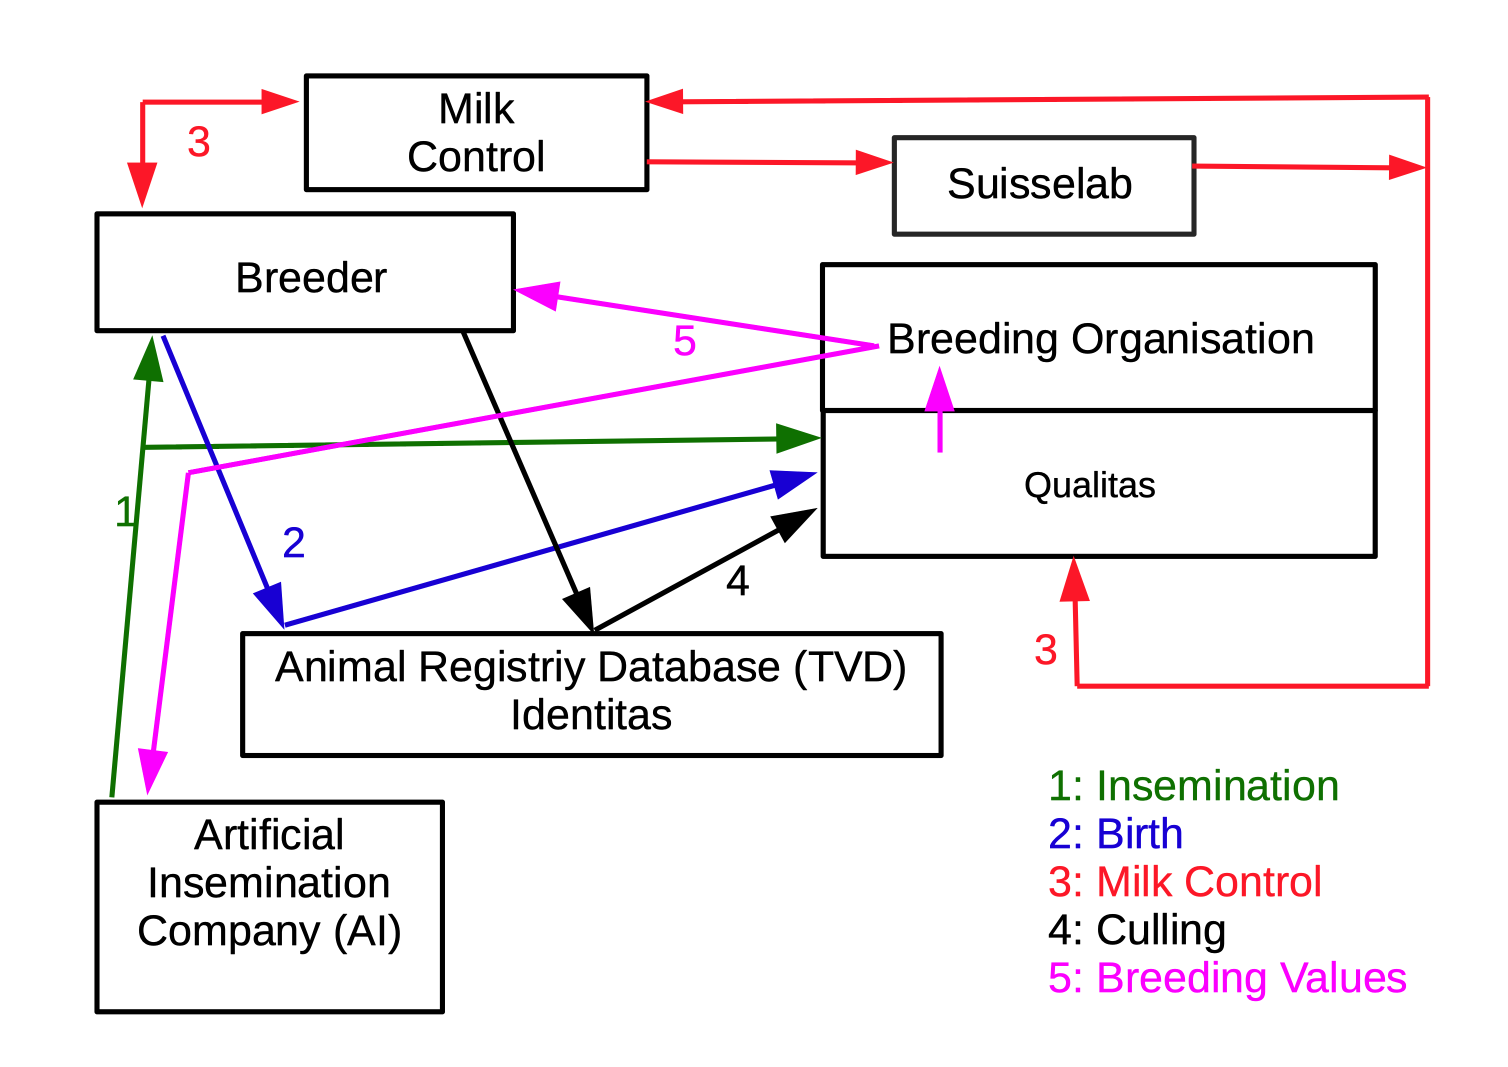
\includegraphics{odg/datacollectionflow.png}
\caption{\label{fig:datacollectionflow}Data Flow in an Animal Breeding Program}
\end{figure}

\hypertarget{asm-genomic-selection}{%
\section{Genomic Selection}\label{asm-genomic-selection}}

The data flow shown in Figure \ref{fig:datacollectionflow} contains the traditional evaluation of data to result in predicted breeding values. But it is missing the newest development in the breeding industry. This development is known as \texttt{Genomic\ Selection} (GS). GS was introduced by the work of \citep{Meuwissen2001}. The methods presented by \citep{Meuwissen2001} were only introduced into practical breeding programs when \citep{Schaeffer2006} showed the tremendous potential of saving costs for breeding programs. The use of \textbf{genomic} information for the assessment of the genetic potential of all breeding animals represents the core of the evaluation approach presented by \citep{Meuwissen2001}. The term \texttt{genomic} is used because genetic markers which are evenly spaced over the complete genome are used as information source. Single Nucleotide Polymorphisms (SNP) are the most widely used marker model nowadays. SNPs are single positions in the genome that occur in different variants in the whole population. A description on how to identify SNPs in a population is given in \citep{Czech2018}. Potential use cases of SNPs are outlined by \citep{SeidelJr.2010} and \citep{Pant2012}. The genetic configuration of an SNP in a given population is shown in Figure \ref{fig:snpgeneticconfiguration}.

\begin{figure}
\centering
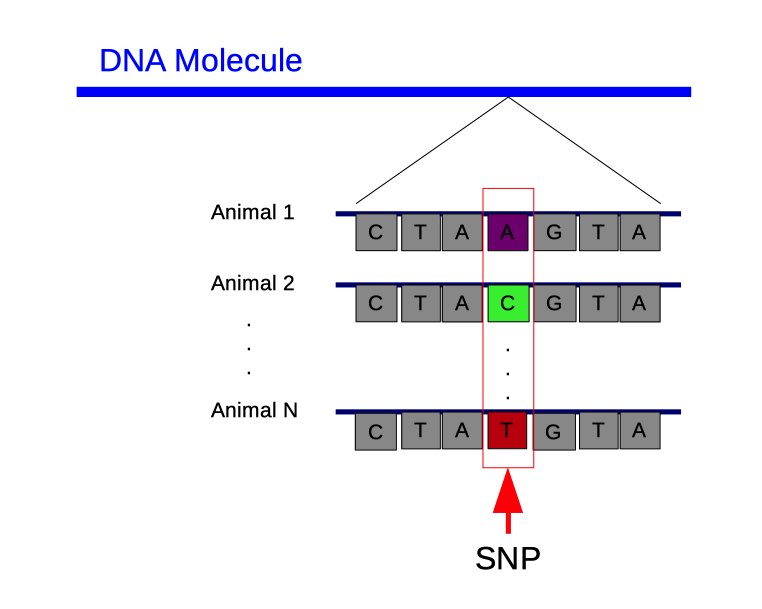
\includegraphics{odg/snpgeneticconfiguration.png}
\caption{\label{fig:snpgeneticconfiguration}Genetic Configuration of a Single Nucleotide Polymorphism (SNP)}
\end{figure}

These SNPs can occur anywhere in the genome which means they can be observed in coding regions, in non-coding regions as well as in regulatory regions. In genomic selection, we are working with a large set of SNPs that are distributed over the complete genome. Hence some of the SNPs will be located close to genetic positions that are important for the expression of quantitative traits of interest. Such genetic positions which are related to quantitative traits are often called \texttt{Quantitative\ Trait\ Loci} (QTL). QTL themselves are difficult to detect and their inheritance is often manifested in complex modes. But due to the likely occurrence of several SNPs in the close proximity of a QTL, the inheritance of QTL alleles and of surrounding SNP alleles will not be independent due to linkage between SNPs and QTL. Such a linkage scenario between two SNPs flanking a QTL is shown in Figure \ref{fig:linkagesnpqtl}.

\begin{figure}
\centering
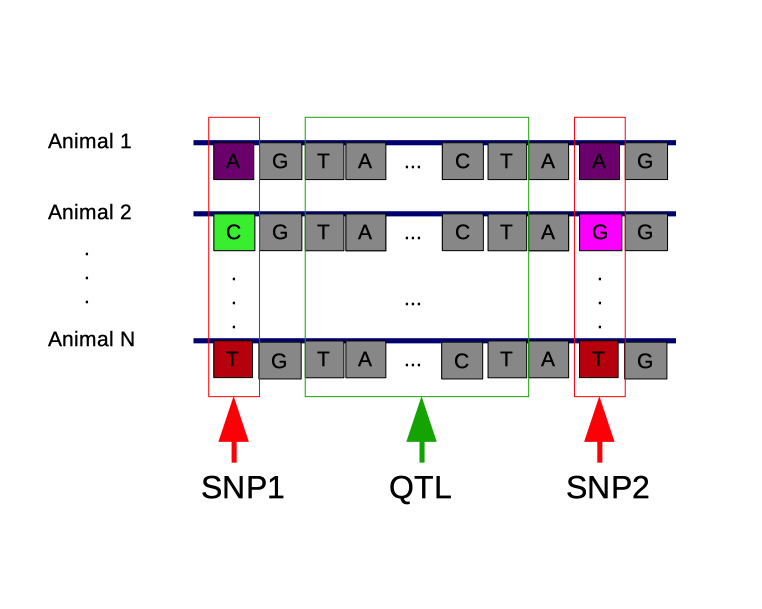
\includegraphics{odg/linkagesnpqtl.png}
\caption{\label{fig:linkagesnpqtl}Two SNPs flanking a QTL}
\end{figure}

Although the QTL is likely to span a range of many positions on the chromosome, we can still assume the QTL to be bi-allelic with alleles \(Q_1\) and \(Q_2\). In theory, any SNP position can have four different alleles according to the four different bases. But when looking at different SNPs in real-world populations, most of them only show two alleles. Hence, for the two SNPs flanking the QTL shown in Figure \ref{fig:linkagesnpqtl} they also have just two alleles \(SNP1_1\), \(SNP1_2\), \(SNP2_1\) and \(SNP2_2\). In genetics the dependency of the inheritance of neighboring loci (marker or QTL) is referred to as \texttt{linkage\ disequilibrium} (LD). This means that any joint allele frequency \(Pr(SNP1_i, Q_j, SNP2_k)\) does not correspond to the product of the single allele frequencies of the two SNPs (\(SNP1\) and \(SNP2\)) and the QTL. In a formula this can be written as

\begin{equation}
 Pr(SNP1_i, Q_j, SNP2_k) \ne Pr(SNP1_i) * Pr(Q_j) * Pr(SNP2_k)
 \label{eq:allelfreqsnpqtllinkage}
\end{equation}

Assuming that the QTL allele \(Q_1\) is favorable for the expression of a given trait of interest and using the fact of LD as expressed in \eqref{eq:allelfreqsnpqtllinkage}, the alleles of \(SNP1\) and \(SNP2\) which occur more frequently together with \(Q_1\) are therefore also related to favorable expression levels of the trait of interest. In real breeding populations, the position of the QTL is unknown. But because we know the allelic configuration of a large number of SNP loci from many breeding animals, we can reliably relate SNP alleles and favorable expression levels of traits of interest.

\hypertarget{asm-mono-genic-model}{%
\section{Mono-Genic Model}\label{asm-mono-genic-model}}

In quantitative genetics, the so-called mono-genic or single-locus model allows us to quantify the genetic potential of breeding animals in terms of breeding values. The standard reference in quantitative genetics in which also the mono-genic model is described is \citep{Falconer1996}. For a single locus, the breeding value depends on the allele frequencies at that locus and on the additive substitution effect which is often called \(\alpha\). The mono-genic model for any given SNP locus in relation to the level of expression of a given trait of interest can be visualized in the following Figure \ref{fig:monogenicsnpmodel}.

\begin{figure}
\centering
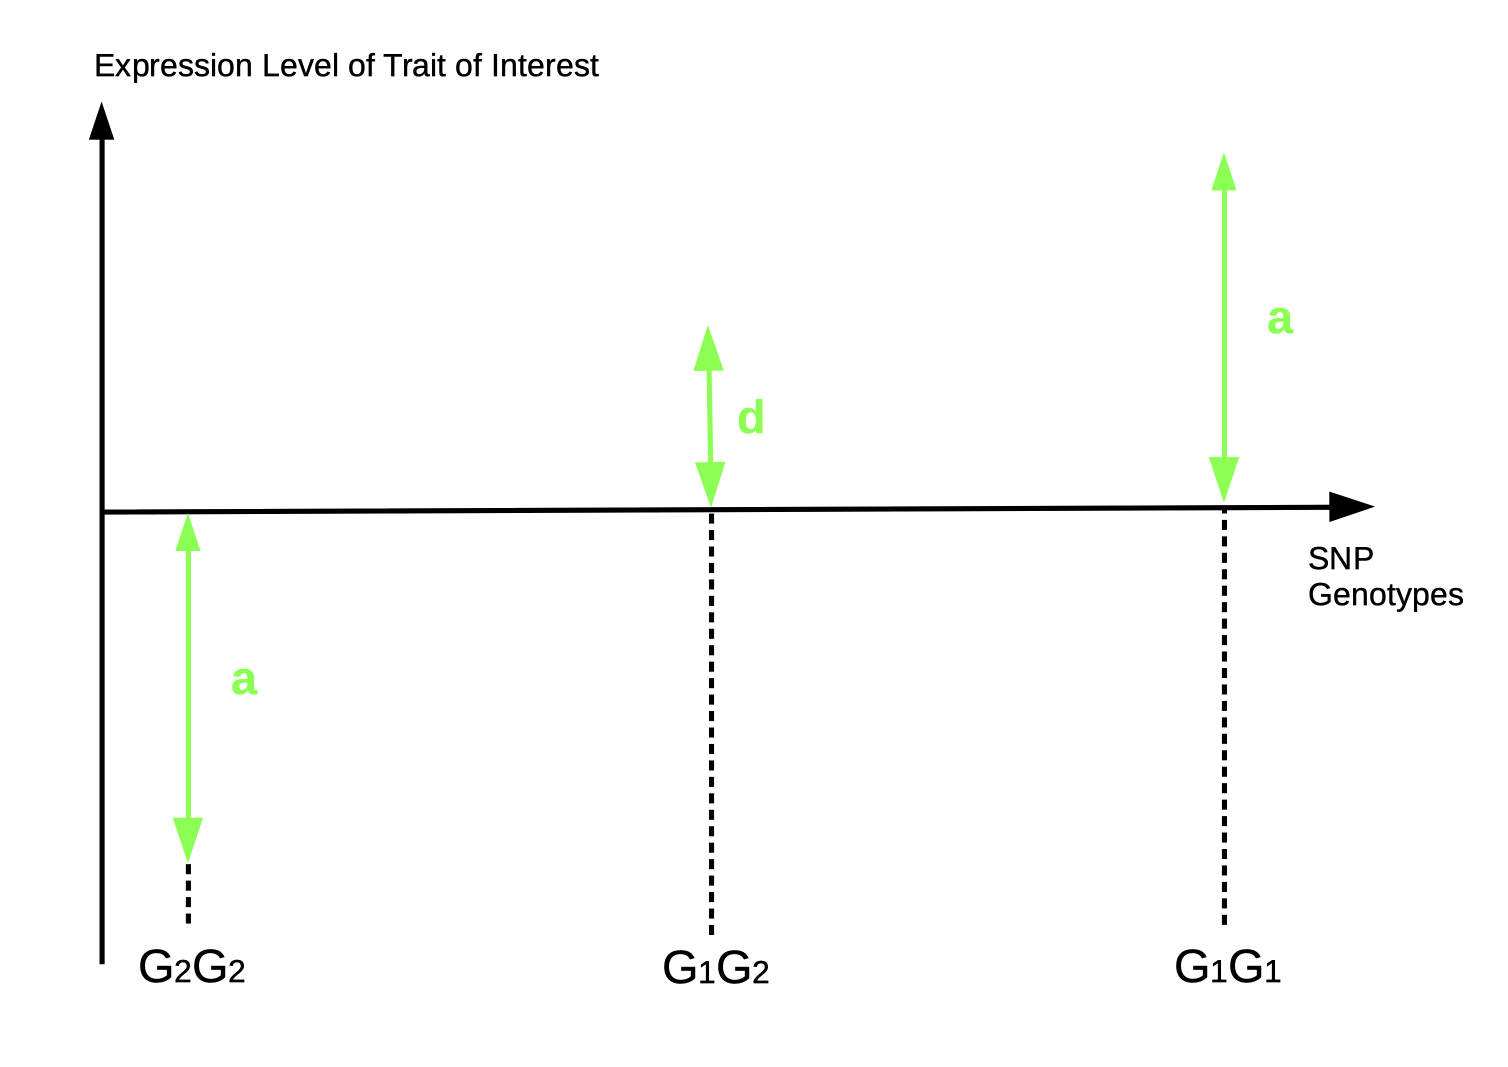
\includegraphics{odg/monogenicsnpmodel.png}
\caption{\label{fig:monogenicsnpmodel}Single-Locus Model for a Quantitative Trait}
\end{figure}

In a real breeding population, we assume that the effect of all loci linked to the SNPs are purely additive. Hence any values for \(d\) are all zero. As a consequence of that the breeding values at any given SNP position only depend on the allele frequencies of the SNP and the \(a\) values at every SNP. The overall breeding value of a given animal is computed as the sum of all locus-specific breeding values. This overall breeding value is called \textbf{genomic breeding value} (GBV). In order to get an estimate of such a GBV, we have to estimate all \(a\) values at any SNP position. This estimation procedure can be done in one of the following two ways.

\begin{enumerate}
\def\labelenumi{\arabic{enumi}.}
\tightlist
\item
  Two step approach
\item
  Single step approach
\end{enumerate}

\hypertarget{asm-two-step-approach}{%
\section{Two Step Approach}\label{asm-two-step-approach}}

In the two step approach the estimation of the \(a\)-values and the computation of the GBVs are done in two separate steps. For the estimation of the \(a\) values for all SNPs, a reference population is defined. In dairy cattle breeding this reference population consists of all male breeding animals. In the recent past, the reference population has been augmented continuously with female animals. The animals in the reference population are all genotyped and they also all have phenotypic measurements\footnote{Whenever phenotypic measurements are not available, traditionally predicted breeding values are transformed back into pseudo phenotypes which are then used to estimate \(a\) values.} for the trait of interest. The estimation of the \(a\) values amounts to estimating fixed effects in a linear model. We will see in later chapters of this course what methods are available to estimate these parameters.

In the second step the estimates for all the \(a\) values are used to compute the GBVs for all animals with genomic SNP information also for those outside of the reference population. The Figure \ref{fig:twostepgs} tries to summarize the process graphically.

\begin{figure}
\centering
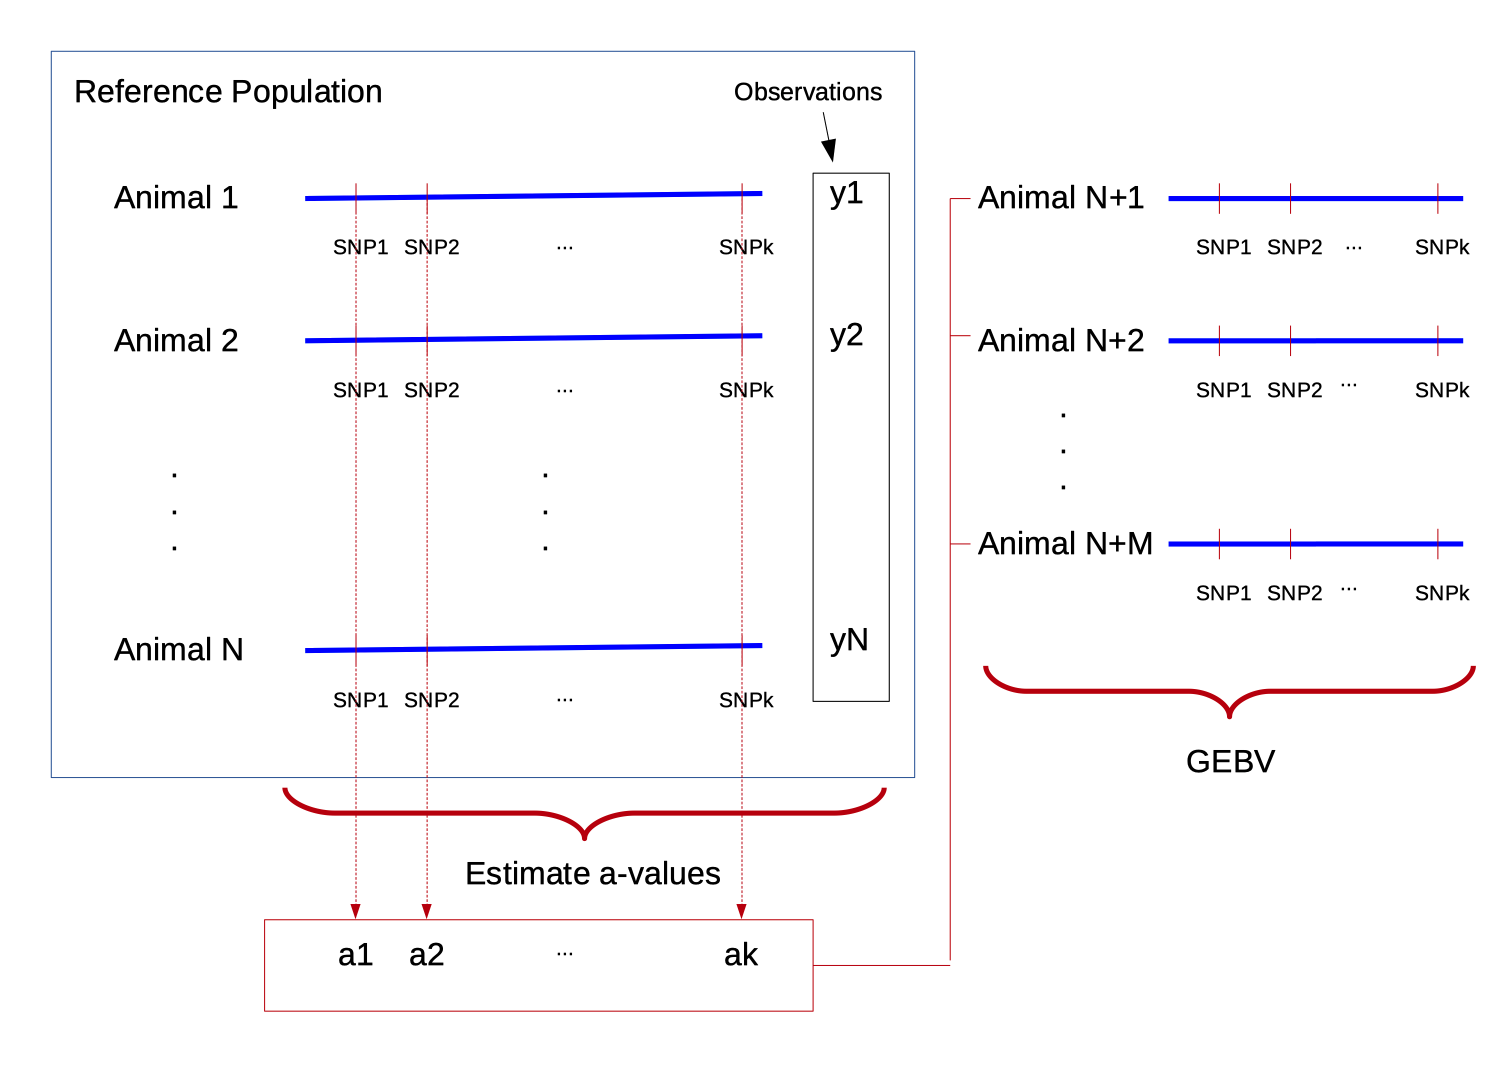
\includegraphics{odg/twostepgs.png}
\caption{\label{fig:twostepgs}Two Step Approach To Estimate Genomic Breeding Values}
\end{figure}

The big advantage of the two step method is that once we have defined a good reference population which yields reliable estimates for the \(a\) values, the computation of the GBV is a simple computation of just summing up the \(a\) contributions with the correct sign determined by the SNP genotypes of the animals for which the GBVs should be determined. All animals with SNP genotypes can get GBV values. The difficult part in the two step approach is to define a reliable reference population and to determine good phenotypic measurements (\(y\)).

\hypertarget{asm-single-step-approach}{%
\section{Single Step Approach}\label{asm-single-step-approach}}

The estimation of the \(a\) values and the prediction of the genomic breeding values is done in one step using linear mixed effects models. In this single step evaluation animals with and without genomic information can get predicted genomic breeding values in a single analysis. One possibility to get to this predicted breeding values is via the use of \texttt{Genomic\ BLUP} (GBLUP). This will be the topic of a complete chapter in this course. The problem with the single step approach is to get an estimate of the covariance between animals with and without genomic information. This is a problem of ongoing research.

\hypertarget{asm-summary}{%
\section{Summary}\label{asm-summary}}

The main difference between traditional predictions of breeding values using a BLUP animal model and the prediction of GBV is that the former uses the so called \textbf{infinitesimal} model to assess the genetic potential and the latter uses sufficiently dense genomic information and uses a \textbf{polygenic} model. This difference is illustrated in Figure \ref{fig:infinitesimalvspolygenic}.

\begin{figure}
\centering
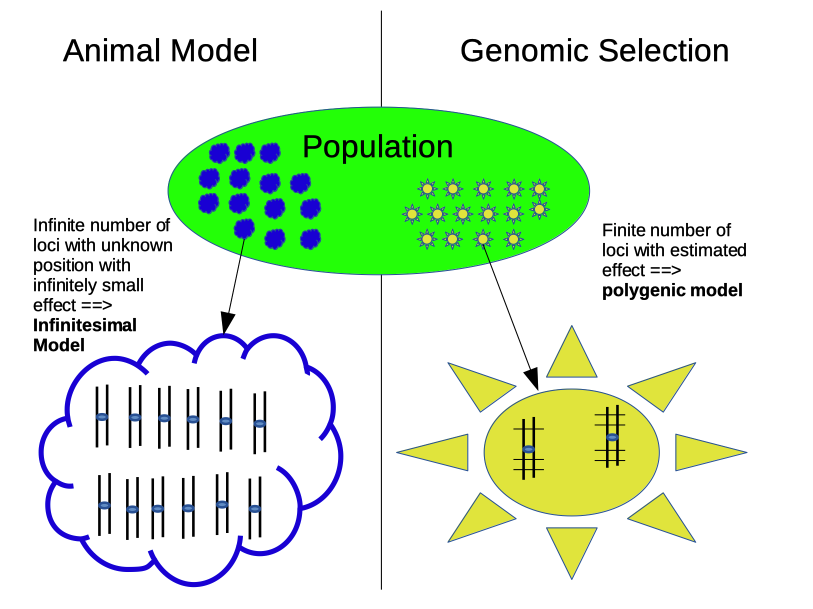
\includegraphics{odg/infinitesimalvspolygenic.png}
\caption{\label{fig:infinitesimalvspolygenic}Infinitesimal Versus Polygenic Model}
\end{figure}

In the remaining chapters, different approaches for the prediction of GBVs are described. Chapter 2 gives a description of the fixed linear effects model and how it was tried to be used for GBV prediction by \citep{Meuwissen2001}. Chapter 3 introduces BLUP methodology in the context of predicting GBVs. In Chapter 4 the method called LASSO is introduced. Interestingly enough, this method is used very seldom in the area of animal breeding. Last but not least, Chapter 5 makes an excursion into Bayesian estimation approaches. The Bayesian methods are important because they are used in practical breeding programs of Swiss Dairy cattle.

\hypertarget{asm-flem}{%
\chapter{Fixed Linear Effects Models}\label{asm-flem}}

\hypertarget{asm-flem-other-resources}{%
\section{Other Resources}\label{asm-flem-other-resources}}

This chapter is based on the work of \citep{Buehlmann2014}. Apart from that there are many other resources for the topic of \texttt{Multiple\ Linear\ Regressions}. An interesting online book is \citep{Lilja2016}.

\hypertarget{asm-flem-motivation}{%
\section{Motivation}\label{asm-flem-motivation}}

Why is the topic of \texttt{fixed\ linear\ effects\ models} (FLEM) important for the analysis of genomic data? This question is best answered when looking at the data. In chapter \ref{asm-intro}, we saw that genomic breeding values can either be estimated using a two-step procedure (see section \ref{asm-two-step-approach}) or by a single step approach (see section \ref{asm-single-step-approach}). At the moment, we assume that we are in the first step of the two step approach where we estimate the marker effects (\(a\)-values) in a reference population or alternatively we have a perfect data set with all animals genotyped and with a phenotypic observation in a single step setting. Both situations are equivalent when it comes to the structure of the underlying dataset and with respect to the proposed model to analyse the data.

\hypertarget{asm-flem-data}{%
\section{Data}\label{asm-flem-data}}

As already mentioned in section \ref{asm-flem-motivation}, we are assuming that we have a perfect data set for a given population of animals. That means each animal \(i\) has a phenotypic observation \(y_i\) for a given trait of interest. Furthermore, we assume to just have a map of three SNP markers. The marker loci are called \(G\), \(H\) and \(I\). Each of the markers has just two alleles. Figure \ref{fig:datastucturegbv} tries to illustrate the structure of a dataset used to estimate GBV.

\begin{figure}
\centering
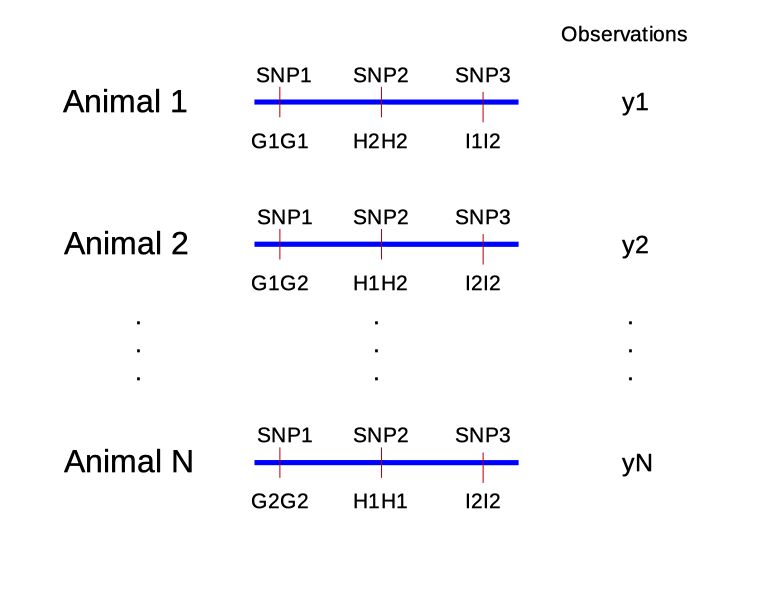
\includegraphics{odg/datastucturegbv.png}
\caption{\label{fig:datastucturegbv}Structure of Dataset To Estimate GBV}
\end{figure}

As can be seen from Figure \ref{fig:datastucturegbv} each of the \(N\) animals have known genotypes for all three SNP markers and they all have a phenotypic observation \(y_i \quad (i = 1, \cdot, N)\). Because we are assuming each SNP marker to be bi-allelic, there are only three possible marker genotypes at every marker position. Hence marker genotypes are discrete entities with a fixed number of levels. Due to the nature of the SNP marker genotype data, we can already say that they could be modeled as fixed effects in a fixed linear effects model. More details about the model will follow in section \ref{asm-flem-model}.

\hypertarget{asm-flem-model}{%
\section{Model}\label{asm-flem-model}}

The goal of our data analysis using the dataset described in section \ref{asm-flem-data} is to come up with estimates for genomic breeding values for all animals in our dataset. The genomic breeding values will later be used to rank the animals. The ranking of the animals according to the GBV is used to select the parents of the future generation of livestock animals. It probably makes sense to distinguish between two different types of models that we have to set up. On the one side we need a model that describes the underlying genetic architecture which is present in our dataset. We will be using a so-called \textbf{genetic} model to describe this. On the other side, we have at some point being able to get estimates for the GBVs which requires a \textbf{statistical} model which is able to estimate unknown parameters as a function of observed data. In the end, we will realize that the two models are actually the same model but they are just different ways of looking at the same structure of underlying phenomena.

\hypertarget{asm-flem-genetic-model}{%
\subsection{Genetic Model}\label{asm-flem-genetic-model}}

The availability of genomic information for all animals in the dataset makes it possible to use a polygenic model. In contrast to an infinitesimal model, a polygenic model uses a finite number of discrete loci to model the genetic part of an expressed phenotypic observation. From quantitative genetics (see e.g. \citep{Falconer1996} for a reference) we know that every phenotypic observation \(y\) can be separated into a genetic part \(g\) and an environmental part \(e\). This leads to the very simple genetic model

\begin{equation}
  y = g + e
  \label{eq:simplegeneticmodel}
\end{equation}

The environmental part can be split into some fixed known systematic factors such as \texttt{herd}, \texttt{season\ effects}, \texttt{age} and more and into a random unknown part. The systematic factors are typically grouped into a vector of fixed effects called \(\beta\). The unknown environmental random part is usually called \(\epsilon\). This allows to re-write the simple genetic model in \eqref{eq:simplegeneticmodel} as

\begin{equation}
  y = \beta + g + \epsilon
  \label{eq:envdecompgeneticmodel}
\end{equation}

The genetic component \(g\) can be decomposed into contributions from the finite number of loci that are influencing the observation \(y\). In our example dataset (see Figure \ref{fig:datastucturegbv}) there are three loci\footnote{Implicitly, we are treating the SNP-markers to be identical with the underlying QTL. But based on the fact that we have very many SNPs spread over the complete genome, there will always be SNP sufficiently close to every QTL that influences a certain trait. But in reality the unknown QTL affect the traits and not the SNPs.} that are assumed to have an effect on \(y\). Ignoring any interaction effects between the three loci, we can decompose the overall genetic effect \(g\) into the some of the genotypic values of each locus. Hence

\begin{equation}
  g = \sum_{j=1}^k g_j
  \label{eq:decompgeneticeffect}
\end{equation}

where for our example \(k\) is equal to three\footnote{In reality \(k\) can be \(1.5*10^5\) for some commercial SNP chip platforms. When working with complete genomic sequences, \(k\) can also be in the order of \(3*10^7\).}.

Considering all SNP loci to be purely additive which means that we are ignoring any dominance effects, the genotypic values \(g_j\) at any locus \(j\) can just take one of the three values \(-a_j\), \(0\) or \(+a_j\) where \(a_j\) corresponds to the \(a\) value from the mono-genic model (see Figure \ref{fig:monogenicsnpmodel}). For our example dataset the genotypic value for each SNP genotype is given in the following table.

\begin{longtable}[t]{lll}
\caption{(\#tab:02-flem-‹›figenotypicvalue)Genotypic Values For All Three SNP-Loci}\\
\toprule
SNP Locus & Genotype & Genotypic Value\\
\midrule
$SNP_1$ & $G_1G_1$ & $a_1$\\
$SNP_1$ & $G_1G_2$ & $0$\\
$SNP_1$ & $G_2G_2$ & $-a_1$\\
$SNP_2$ & $H_1H_1$ & $a_2$\\
$SNP_2$ & $H_1H_2$ & $0$\\
\addlinespace
$SNP_2$ & $H_2H_2$ & $-a_2$\\
$SNP_3$ & $I_1I_1$ & $a_3$\\
$SNP_3$ & $I_1I_2$ & $0$\\
$SNP_3$ & $I_2I_2$ & $-a_3$\\
\bottomrule
\end{longtable}

From the Table \ref{tab:genotypicvalue} we can see that always the allele with subscript \(1\) is taken to be that with the positive effect. Combining the information from Table \ref{tab:genotypicvalue} together with the decomposition of the genotypic value \(g\) in \eqref{eq:decompgeneticeffect}, we get

\begin{equation}
  g = M \cdot a
  \label{eq:genotypicvalueintermsofa}
\end{equation}

where \(M\) is an indicator matrix taking values of \(-1\), \(0\) and \(1\) depending on the SNP marker genotype and \(a\) is a vector of \(a\) values. Combining the decomposition in \eqref{eq:genotypicvalueintermsofa} together with the basic genetic model in \eqref{eq:envdecompgeneticmodel}, we get

\begin{equation}
  y = \beta + M \cdot a + \epsilon
  \label{eq:finalgeneticmodel}
\end{equation}

The result obtained in \eqref{eq:envdecompgeneticmodel} is the fundamental decomposition of the phenotypic observation \(y\) into a genetic part represented by the SNP marker information (\(M\)) and an environmental part (\(\beta\) and \(\epsilon\)). The \(a\) values are unknown an must be estimated. The estimates of the \(a\) values will then be used to predict the GBVs. How this estimation procedure works is described in the next section \ref{asm-flem-statistical-model}.

\hypertarget{asm-flem-statistical-model}{%
\subsection{Statistical Model}\label{asm-flem-statistical-model}}

When looking at the fundamental decomposition given in the genetic model presented in \eqref{eq:finalgeneticmodel} from a statistics point of view, the model in \eqref{eq:finalgeneticmodel} can be interpreted as \textbf{fixed linear effects model} (FLEM). FLEM represent a class of linear models where each model term except for the random residual term is a fixed effect. Furthermore, besides a random error term, the response is explained by a linear function of the predictor variables.

Using the decomposition given in our genetic model (see equation \eqref{eq:finalgeneticmodel}) for our example dataset illustrated in Figure \ref{fig:datastucturegbv}, every observation \(y_i\) of animal \(i\) can be written as

\begin{equation}
  y_i = W_i \cdot \beta + M_i \cdot a + \epsilon_i
  \label{eq:basisstatisticalmodel}
\end{equation}

where

\begin{itemize}
\tightlist
\item
  \(y_i\) is the observation of animal \(i\)
\item
  \(\beta\) is a vector of unknown systematic environmental effects
\item
  \(W_i\) is an indicator row vector linking \(\beta\) to \(y_i\)
\item
  \(a\) is a vector of unknown additive allele substitution effects (\(a\) values)
\item
  \(M_i\) is an indicator row vector encoding the SNP genotypes of animal \(i\) and
\item
  \(\epsilon_i\) is the random unknown environmental term belonging to animal \(i\)
\end{itemize}

In the following section, we write down the definition of a FLEM and compare it to the statistical model given in \eqref{eq:basisstatisticalmodel}.

\hypertarget{asm-flem-definition}{%
\section{Definition of FLEM}\label{asm-flem-definition}}

The multiple fixed linear effects model is defined as follows.

\BeginKnitrBlock{definition}[Fixed Linear Effects Model]
\protect\hypertarget{def:defflem}{}{\label{def:defflem} \iffalse (Fixed Linear Effects Model) \fi{} }In a fixed linear effects model, every observation \(i\) in a dataset is characterized by a \textbf{response variable} and a set of \textbf{predictors}. Up to some random errors the response variable can be expressed as a linear function of the predictors. The proposed linear function contains unknown parameters. The goal is to estimate both the unknown parameters and the error variance.
\EndKnitrBlock{definition}

\hypertarget{asm-flem-terminology}{%
\subsection{Terminology}\label{asm-flem-terminology}}

For datasets where both the predictors and the response variables are on a continuous scale, which means that they correspond to measured quantities such as body weight, breast circumference or milk yield, the model is referred to as \textbf{multiple linear regression model}. Because the statistical model in \eqref{eq:basisstatisticalmodel} contains the SNP genotypes as discrete fixed effects, we are not dealing with a regression model but with a more general fixed linear effects model.

\hypertarget{asm-flem-model-specification}{%
\subsection{Model Specification}\label{asm-flem-model-specification}}

An analysis of the model given in \eqref{eq:basisstatisticalmodel} shows that it exactly corresponds to the definition \ref{def:defflem}. In this equivalence, the observation \(y_i\) corresponds to the response variable. Furthermore, the unknown environmental term \(\epsilon\) corresponds to the random residual part in the FLEM. Except for the random residuals the response variable \(y_i\) is a linear function of the fixed effects which corresponds to all systematic environmental effects and to all SNP genotype effects.

For the description of how to estimate the unknown parameter \(\beta\) and \(a\) in the model \eqref{eq:basisstatisticalmodel}, it is useful to combine \(\beta\) and \(a\) into a single vector of unknown parameters and we call it \(b\).

\begin{equation}
  b = \left[ \begin{array}{c} \beta \\ a \end{array} \right]
  \label{eq:combinefixedeffects}
\end{equation}

Taking the equations as shown in \eqref{eq:basisstatisticalmodel} for all observations (\(i=1, \ldots, N\)) and expressing them in matrix-vector notation, we get

\begin{equation}
 y = Xb + \epsilon
 \label{eq:flemmatrixvector}
\end{equation}

where

\begin{itemize}
\tightlist
\item
  \(y\) is the vector of \(N\) observations
\item
  \(b\) is the vector of all unknown fixed effects
\item
  \(X\) is the incidence matrix linking the parameters of \(b\) to \(y\)
\item
  \(\epsilon\) is the vector of random residuals
\end{itemize}

The incidence matrix \(X\) in \eqref{eq:flemmatrixvector} can be composed from the matrices \(W\) and \(M\) by concatenating the latter two matrices, i.e.,

\begin{equation}
  X = \left[ \begin{array}{cc} W  &  M  \end{array} \right]
  \label{eq:composematrixx}
\end{equation}

\hypertarget{asm-flem-parameter-estimation}{%
\section{Parameter Estimation Using Least Squares}\label{asm-flem-parameter-estimation}}

The method of parameter estimation is explained using the simpler case of a regression model. That means both the predictors and the response variables are on a continuous scale. As a further simplification, we assume that there is only one predictor variable and one response variable. The predictor variable is called \(x\) and the response variable is called \(y\). The model is still the same as shown in \eqref{eq:flemmatrixvector}. The matrix \(X\) has just one column with the measured values of the predictor variable and \(b\) is just a scalar unknown parameter. The vector \(y\) contains the observed values for the response values.

The goal of the analysis of the simple dataset is to find an estimate of the scalar \(b\) such that the linear combination of \(X\) and \(b\) best explains the values in \(y\). How we can find such an estimation procedure that allows us to calculate an estimate of \(b\) is explained using a small example data set in the following subsection.

\hypertarget{asm-flem-regression-example}{%
\subsection{An Example Dataset}\label{asm-flem-regression-example}}

A widely use example dataset for such a simple regression analysis in animal breeding consists of measurements of \texttt{body\ weight} (BW) and \texttt{breast\ circumference} (BC) for a given group of animals.

\begin{longtable}[t]{rrr}
\caption{\label{tab:dataregression}Dataset for Regression of Body Weight on Breast Circumference for ten Animals}\\
\toprule
Animal & Breast Circumference & Body Weight\\
\midrule
1 & 176 & 471\\
2 & 177 & 463\\
3 & 178 & 481\\
4 & 179 & 470\\
5 & 179 & 496\\
\addlinespace
6 & 180 & 491\\
7 & 181 & 518\\
8 & 182 & 511\\
9 & 183 & 510\\
10 & 184 & 541\\
\bottomrule
\end{longtable}

The dataset shown above is taken from Table 9.1 in \citep{Essl1987}. One of the possible reasons for fitting a regression from BW on BC is that the latter is easier to measure. The measured values of BC can be used to predict BW once we have determined the regression coefficient. For this prediction, we use BW as response variable \(y\) and BC as predictor variable \(x\). This leads to the regression model

\begin{equation}
  y = x * b + \epsilon
  \label{eq:regressionbwonbc}
\end{equation}

where \(y\) is the vector of body weights and \(x\) is the vector of breast circumferences. \(b\) is a scalar value which is unknown and \(\epsilon\) is the vector of random unknown error terms. The goal is to determine \(b\) such that the predictor variable best explains the response variable. How \(b\) is determined is explained with the following plot.

\begin{figure}
\centering
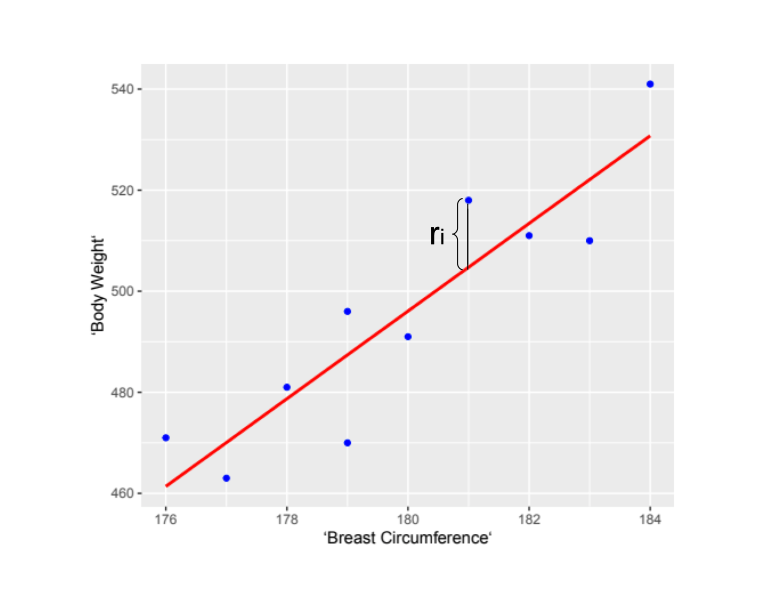
\includegraphics{odg/showregressionbwonbc.png}
\caption{\label{fig:showregressionbwonbc}Regression of Body Weight On Breast Circumference}
\end{figure}

In Figure \ref{fig:showregressionbwonbc} the blue points correspond to the data points given by the dataset shown in Table \ref{tab:dataregression}. The red line corresponds to the regression line defined by the unknown regression parameter \(b\). The distance between the data points to the projection in the direction of the \(y\)-axis corresponds to the residual \(r\). For a given data point \(i\), the residual \(r_i\) is computed as

\begin{equation}
  r_i = y_i - x_i * \hat{b}
  \label{eq:definitionresidual}
\end{equation}

where \(\hat{b}\) denotes a concrete estimated value of \(b\). For a different choice of a value of \(\hat{b}\), different values for the residuals \(r_i\) can be computed. Our goal is to find the value of \(\hat{b}\) that results in the smallest residuals \(r_i\). In order to avoid cancellation of positive and negative values of the residuals, the \(r_i\) values are squared and added. This sum of the squared residuals is used as a measure of how good a given regression line determined by \(\hat{b}\) fits a given set of data points. Because we want to have a good fit this means that the sum of the squared residuals should be as small as possible.

The method that determines \(\hat{b}\) such that the sum of the squared residuals is minimal is called \textbf{Least Squares}. In a general formula with more than one predictor variables we can write the least squares estimate \(\hat{b}_{LS}\) as

\begin{equation}
  \hat{b}_{LS} = argmin_b ||y - Xb||^2
  \label{eq:leastsquaresestimate}
\end{equation}

where \(||.||\) denotes the Euclidean norm. The estimate \(\hat{b}_{LS}\) can be found by finding the minimum of \(||y - Xb||^2\). The minimum of \(||y - Xb||^2\) is found by first taking the derivative with respect to \(b\) and the setting that derivative to \(0\). The derivative of \(||y - Xb||^2\) with respect to \(b\) can be computed as follows

\begin{equation}
  LS = ||y - Xb||^2 = (y - Xb)^T(y - Xb) = y^Ty - y^TXb - b^TX^Ty + b^TX^TXb
  \label{eq:computels}
\end{equation}

The derivative of \(LS\) with respect to \(b\) is

\begin{equation}
  \frac{\partial LS}{\partial b} = -y^TX - y^TX + 2*b^TX^TX
  \label{eq:partiallswrtb}
\end{equation}

The minimum is found by setting \(\frac{\partial LS}{\partial b}\) to \(0\).

\begin{equation}
  \frac{\partial LS}{\partial b} = -y^TX - y^TX + 2*\hat{b}^TX^TX = 0
  \label{eq:minimumls}
\end{equation}

From equation \eqref{eq:minimumls}, we get the so-called least squares \textbf{Normal Equations} for \(\hat{b}\).

\begin{equation}
   X^TX\hat{b} = X^Ty
  \label{eq:lsnormalequations}
\end{equation}

For a regression model, we know that \(X\) has full column rank\footnote{In a regression model, all values in the matrix \(X\) are real values. Hence no column of \(X\) will be a linear combination of any other columns and therefore \(X\) has full column rank.}. That means we can solve the normal equations \eqref{eq:lsnormalequations} explicitly for \(\hat{b}\).

\begin{equation}
   \hat{b} = (X^TX)^{-1}X^Ty
  \label{eq:solutionhatb}
\end{equation}

Equation \eqref{eq:solutionhatb} presents a solution to the estimation problem of the unknown parameter \(b\) in the regression problem. There is one additional unknown parameter that we have not mentioned so far. The regression model contains the random error terms \(\epsilon\). Because \(\epsilon\) is random, we have to specify the expected value and the variance. The error terms are deviations of the predicted values from the observed data points. Hence the expected values \(E\left[\epsilon \right]\) must be \(0\). The variance \(\sigma^2\) of the error terms is an additional unknown parameter that has to be estimated from the data. One way of estimating the error variance from the data is shown in subsection \ref{asm-flem-error-variance}.

\hypertarget{asm-flem-error-variance}{%
\subsection{Variance of Errors}\label{asm-flem-error-variance}}

The least squares procedure itself does not yield an estimate of the error variance \(\sigma^2\). But the estimate of \(\sigma^2\) based on the residuals is often declared to be the \texttt{least\ squares\ estimate} of \(\sigma^2\). The residuals \(r_i\) as defined in \eqref{eq:definitionresidual} are estimates of the error terms \(\epsilon_i\). As a matter of fact the residuals can be used to estimate \(\sigma^2\). This estimate is given by

\begin{equation}
  \widehat{\sigma^2} = \frac{1}{n-p} \sum_{i=1}^n r_i^2
  \label{eq:lsestimateerrorvariance}
\end{equation}

The factor \((n-p)^{-1}\) in \eqref{eq:lsestimateerrorvariance} is used, because it leads the estimate \(\widehat{\sigma^2}\) to be unbiased, which means \(E\left[\widehat{\sigma^2} \right] = \sigma^2\).

\hypertarget{asm-flem-types-of-regression}{%
\section{Different Types of Linear Regressions}\label{asm-flem-types-of-regression}}

\hypertarget{asm-flem-regression-origin}{%
\subsection{Regression Through The Origin}\label{asm-flem-regression-origin}}

The regression model as it was proposed in \eqref{eq:regressionbwonbc} for the dataset of body weight and breast circumference defines a line in the \(x-y\)-plane. This line shown in Figure \ref{fig:showregressionbwonbc}. What is not shown in the plot, but what becomes clear from the model is that the regression line goes through the origin of the coordinate system. Mathematically the origin is given by \(x=0\) and \(y=0\). In this regression model, the origin is the fixed point which is on the regression line. The fixed point together with the estimated regression coefficient \(\hat{b}\) uniquely define the regression line. From a geometrical point of view the estimated regression coefficient defines the slope of the regression line.

\hypertarget{asm-flem-regression-intercept}{%
\subsection{Regression With Intercept}\label{asm-flem-regression-intercept}}

Depending on the data analysed with a regression model, it does not make sense to force the regression line to run through the origin. This can be avoided by including an additional fixed term in the regression model. This term is called the \textbf{intercept}. A regression model with an intercept can be written as

\begin{equation}
  y_i = b_0 + x_i * b_1 + \epsilon_i
  \label{eq:regressionintercept}
\end{equation}

The term \(b_0\) corresponds to the value of the response variable \(y\) when the value of the predictor \(x\) is \(0\). Then the fixed point of the regression line is no longer the origin, but the point \(x = 0\) and \(y = \widehat{b_0}\). The slope of the regression line is determined by \(\widehat{b_1}\). In matrix-vector notation the intercept \(b_0\) is added to the vector of unknown parameters \(b\) and the design-matrix \(X\) has to be augmented by a column of all ones on the left.

\hypertarget{asm-flem-regression-transformed-predictors}{%
\subsection{Regression With Transformed Predictor Variables}\label{asm-flem-regression-transformed-predictors}}

Regression models can also contain different transformations of the predictor variables. As an example, we can include any higher order polynomial functions of predictor variables such as

\begin{equation}
  y_i = b_0 + b_1 * x_i + b_2 * x_i^2 + \cdots + b_k * x_i^k + \epsilon_i
  \label{eq:polynomialregression}
\end{equation}

Although the model \eqref{eq:polynomialregression} contains non-linear functions of the predictors \(x_i\), the function is still linear in the unknown parameters \(b_j\) (\(j = 1, \ldots k\)) and hence the model \eqref{eq:polynomialregression} is still a linear regression model.

Transformations of the predictor variables are not restricted to polynomial functions. Many different kinds of transformations are possible. An example is shown in the following equation

\begin{equation}
  y_i = b_0 + b_1 * log(x_i) + b_2 * sin(\pi x_i) + \epsilon_i
  \label{eq:generalregression}
\end{equation}

\hypertarget{asm-flem-prediction}{%
\section{Predictions}\label{asm-flem-prediction}}

One goal of estimating the regression coefficient was that we want to be able to predict the response based on concrete values of the predictor variables. For our example with the body weight and the breast circumference, this means that we want to measure the breast circumference of an animal for which we do not know the body weight. Then based on the estimated regression coefficient, we want to be able to predict the body weight of that animal.

The computation of the regression coefficient for the dataset shown in Table \ref{tab:dataregression} will be the topic of an exercise. But let us assume that we have computed the value of \(\hat{b}\), then the predicted value of the body weight \(\widehat{y_s}\) for an animal \(s\) is computed based on the measured breast circumference \(x_s\) of animal \(s\) as follows

\begin{equation}
  \widehat{y_s} = \hat{b} * x_s
  \label{eq:predictbwonbc}
\end{equation}

It has to be noted that the prediction \(\widehat{y_s}\) is only valid, if the measured value \(x_s\) is close to the measured predictors that were used to estimate \(\hat{b}\). For our example with body weight and breast circumference, we could not use the same regression line to predict the body weight for calves, if \(\hat{b}\) was estimated with data of adult bulls.

\hypertarget{asm-flem-reg-dummy}{%
\section{Regression On Dummy Variables}\label{asm-flem-reg-dummy}}

In a regression model (such as shown in \eqref{eq:regressionbwonbc}) both the response variable and the predictor variables are continuous variables. Examples of such variables are \texttt{body\ weight} and \texttt{breast\ circumference} which are both measured and the measurements are expressed as real numbers. In contrast to such a regression model, the statistical model shown in \eqref{eq:basisstatisticalmodel} has a continuous response, but the predictor variables are discrete variables. The predictor variables are assumed to be genotypes of a certain set of SNP genotypes and hence these genotypes can only have a fixed number of states. Under the assumption of bi-allelic Loci, a SNP locus can have just three genotypes and hence the predictor variable that is used to represent any given SNP-locus can only take three discrete states.

Figure \ref{fig:compareregflem} shows the difference between a regression model as the one of \texttt{body\ weight} on \texttt{breast\ circumference} and a fixed linear effects model where one locus has an effect on a quantitative trait. In the left diagram of Figure \ref{fig:compareregflem} the red line denotes the regression line. This line is meaningful because on the x-axis and on the y-axis every single point of the red line would be valid observations. On the x-axis of the diagram on the righthand side, only three values are possible. In the diagram they are shown as Genotypes \(G_1G_1\), \(G_1G_2\) and \(G_2G_2\). We will see very soon that in our statistical model, they will be encoded by \(1\), \(0\) and \(-1\). The response variable in the diagram on the right of Figure \ref{fig:compareregflem} is a continuous random variable, similarly to the regression model shown in the left diagram. This combination of continuous response variable on a discrete type of variable lead to the term \textbf{regression on dummy variables} because the predictor variables are not continuous but just discrete levels of a certain factor. In this lecture, we are using \textbf{fixed linear effects model} rather than regression on dummy variables for the same type of model. The term of fixed linear effects model was used, because in the next chapter in Genomic BLUP we are going to introduce mixed linear effects model which are an extension of the fixed linear effects model used in this chapter.

\begin{figure}
\centering
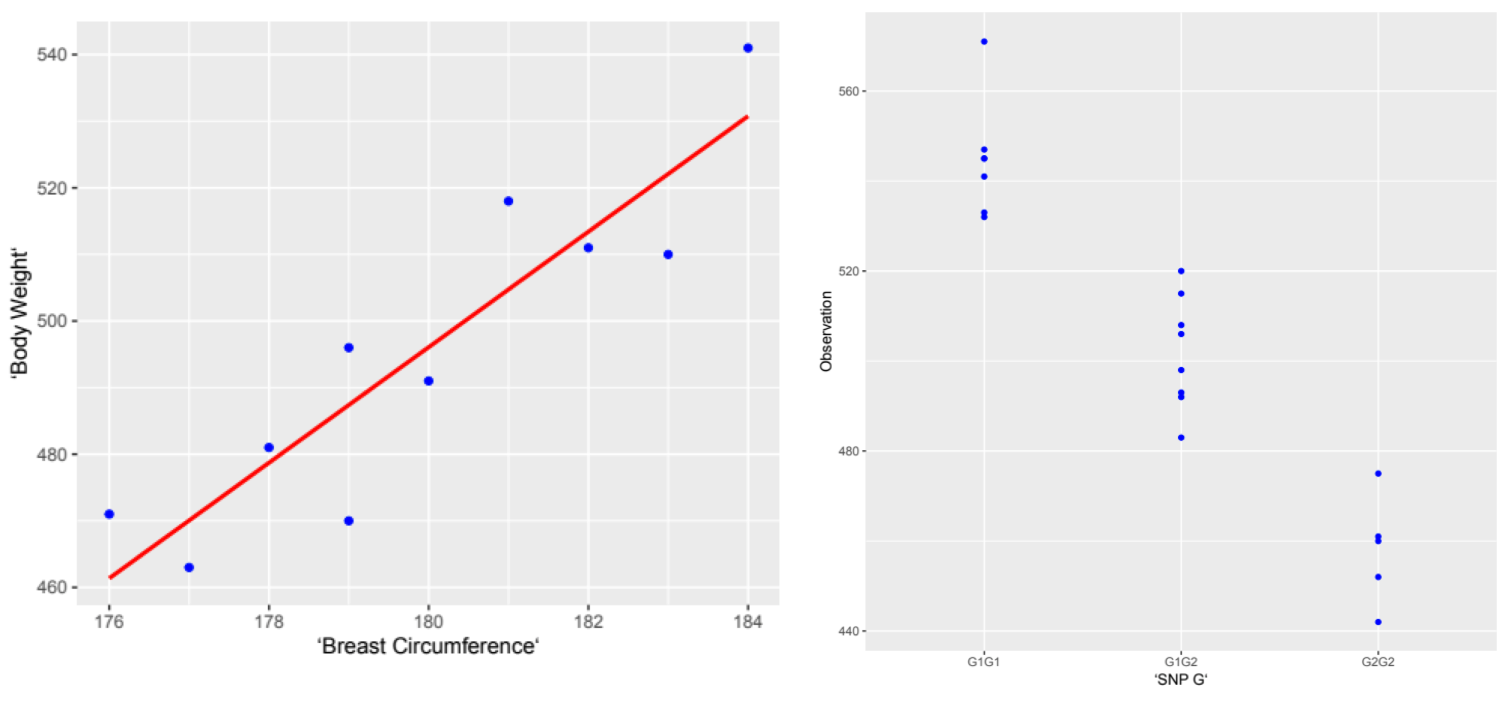
\includegraphics{odg/compareregflem.png}
\caption{\label{fig:compareregflem}Comparison Between Regression Model And Fixed Linear Effects Model With An SNP-Locus As A Discrete Predictor Variables}
\end{figure}

\hypertarget{asm-flem-flem-for-snp}{%
\subsection{Fixed Linear Effects Model For SNP Data}\label{asm-flem-flem-for-snp}}

We are using genetic data and assume that the SNP genotypes have an effect on a quantitative trait. Our goal is to predict genomic breeding values based on the information from the SNP genotypes for the quantitative traits. We have seen that under some simplifying assumptions of additivity of the genetic effects, the genomic breeding values depend on the absolute value of the genotypic values (\(a\) values) of the homozygous SNP genotypes. Hence all we need to know from our analysis of the data under a fixed linear effects model are the \(a\) values for each SNP locus. The decomposition of the phenotypic observation shown in \ref{asm-flem-genetic-model} under the assumed genetic model tells us that the phenotypic observation can be explained as a linear function of the genotypic values of the SNP genotypes plus a random error term. The fact that our genetic model is a fixed linear effects model that uses phenotypic observations as response and SNP loci as predictors allows us to set up the following model for an example data set shown in the following subsection.

\hypertarget{asm-flem-snp-obs}{%
\subsection{Example Data Set With SNP Loci And A Phenotypic Observation}\label{asm-flem-snp-obs}}

We are using the dataset shown in Table \ref{tab:dataflemsnpobs} as an example on how to use a fixed linear effects model to estimate the genotypic value of the SNP genotypes.

\begin{table}

\caption{\label{tab:dataflemsnpobs}Animals With Two SNP Loci Affecting A Quantitative Trait}
\centering
\begin{tabular}[t]{rllllr}
\toprule
Animal & SNP G & Genotypic Value G & SNP H & Genotypic Value H & Observation\\
\midrule
1 & $G_1G_1$ & $a_G$ & $H_1H_2$ & $0$ & 510\\
2 & $G_1G_2$ & $0$ & $H_1H_1$ & $a_H$ & 528\\
3 & $G_1G_2$ & $0$ & $H_1H_1$ & $a_H$ & 505\\
4 & $G_1G_1$ & $a_G$ & $H_2H_2$ & $-a_H$ & 539\\
5 & $G_1G_1$ & $a_G$ & $H_1H_1$ & $a_H$ & 530\\
\addlinespace
6 & $G_1G_2$ & $0$ & $H_1H_2$ & $0$ & 489\\
7 & $G_1G_2$ & $0$ & $H_2H_2$ & $-a_H$ & 486\\
8 & $G_2G_2$ & $-a_G$ & $H_1H_1$ & $a_H$ & 485\\
9 & $G_1G_2$ & $0$ & $H_2H_2$ & $-a_H$ & 478\\
10 & $G_2G_2$ & $-a_G$ & $H_1H_2$ & $0$ & 479\\
\addlinespace
11 & $G_1G_1$ & $a_G$ & $H_1H_2$ & $0$ & 520\\
12 & $G_1G_1$ & $a_G$ & $H_1H_1$ & $a_H$ & 521\\
13 & $G_2G_2$ & $-a_G$ & $H_1H_2$ & $0$ & 473\\
14 & $G_2G_2$ & $-a_G$ & $H_1H_2$ & $0$ & 457\\
15 & $G_1G_2$ & $0$ & $H_1H_1$ & $a_H$ & 497\\
\addlinespace
16 & $G_1G_2$ & $0$ & $H_1H_2$ & $0$ & 516\\
17 & $G_1G_1$ & $a_G$ & $H_1H_2$ & $0$ & 524\\
18 & $G_1G_1$ & $a_G$ & $H_1H_2$ & $0$ & 502\\
19 & $G_1G_1$ & $a_G$ & $H_2H_2$ & $-a_H$ & 508\\
20 & $G_1G_2$ & $0$ & $H_1H_2$ & $0$ & 506\\
\bottomrule
\end{tabular}
\end{table}

Instead of fitting individual effects for the different SNP genotypes to explain the response variable, we are directly including the genotypic values \(a_G\) and \(a_H\) into the fixed effects linear model. How the genotypic values are related to the SNP genotypes is also shown in Table \ref{tab:dataflemsnpobs}. For all animals in Table \ref{tab:dataflemsnpobs}, we can write the model equations in matrix-vector notation as

\begin{equation}
  y = Xb + \epsilon
  \label{eq:flemsnp}
\end{equation}

where \(y\) is the vector of observations, \(b\) is a vector of genotypic values plus an intercept, \(X\) is a design matrix linking the elements in \(b\) to \(y\) and \(\epsilon\) is a vector of random errors. Writing out the matrices and vectors leads to

\begin{equation}
\left[\begin{array}{r}
  510 \\ 
  528 \\ 
  505 \\ 
  539 \\ 
  530 \\ 
  489 \\ 
  486 \\ 
  485 \\ 
  478 \\ 
  479 \\ 
  520 \\ 
  521 \\ 
  473 \\ 
  457 \\ 
  497 \\ 
  516 \\ 
  524 \\ 
  502 \\ 
  508 \\ 
  506 \\ 
  \end{array} 
\right]
 = 
\left[\begin{array}{rrr}
  1 & 1 & 0 \\ 
  1 & 0 & 1 \\ 
  1 & 0 & 1 \\ 
  1 & 1 & -1 \\ 
  1 & 1 & 1 \\ 
  1 & 0 & 0 \\ 
  1 & 0 & -1 \\ 
  1 & -1 & 1 \\ 
  1 & 0 & -1 \\ 
  1 & -1 & 0 \\ 
  1 & 1 & 0 \\ 
  1 & 1 & 1 \\ 
  1 & -1 & 0 \\ 
  1 & -1 & 0 \\ 
  1 & 0 & 1 \\ 
  1 & 0 & 0 \\ 
  1 & 1 & 0 \\ 
  1 & 1 & 0 \\ 
  1 & 1 & -1 \\ 
  1 & 0 & 0 \\ 
  \end{array} 
\right]
\left[\centering
\begin{array}{l}
  b_0 \\ 
  a_G \\ 
  a_H \\ 
  \end{array} 
\right]
 + \epsilon\end{equation}

\hypertarget{asm-flem-parameter-estimation}{%
\subsection{Parameter Estimation In A Fixed Linear Effects Model}\label{asm-flem-parameter-estimation}}

The goal for model \eqref{eq:flemsnp} is to get an estimate for the unknown parameters \(b_0\), \(a_G\) and \(a_H\). In section \ref{asm-flem-parameter-estimation} we saw how unknown parameters can be estimated for a regression model using least squares. When applying the least squares method, we did not make any assumptions about the predictor variables. The minimization of the sum of the squared residuals can also be applied for the fixed linear effects model. This minimization leads to the same normal equations

\begin{equation}
  X^TXb^{(0)} = X^Ty
  \label{eq:normalequationflem}
\end{equation}

So far everything was identical to the case of the regression model. But when trying to find a solution for \eqref{eq:normalequationflem} we have to account for the different nature of the design matrix \(X\). In the regression model this matrix \(X\) contains real numbers. In our example of a fixed linear effects model, the matrix \(X\) just contains just the three number \(-1\), \(0\) and \(1\)\footnote{In most other fixed linear effects models, the design matrix contains just \(0\) and \(1\).}. The fact that the matrix \(X\) contains only a few discrete values makes it very likely that \(X\) does not have full column rank. That means it is very likely that some columns of \(X\) can be expressed as linear combinations of other columns. This linear dependence of the columns of \(X\) causes the matrix \(X^TX\) to be singular and hence the inverse of \(X^TX\) cannot be computed. Whenever the matrix \(X^TX\) is singular, the solution given in \eqref{eq:solutionhatb} cannot be computed.

The normal equations in \eqref{eq:normalequationflem} are written with the symbol \(b^{(0)}\) to denote that the equations do not have a single solution \(b^{(0)}\) in the sense that we were able to compute them in the case of the regression model. In the case where \(X^TX\) is singular, there are infinitely many solutions \(b^{(0)}\). These solutions can be expressed as

\begin{equation}
  b^{(0)} = (X^TX)^-X^Ty
  \label{eq:gensolnormalequationflem}
\end{equation}

where \((X^TX)^-\) stands for a \textbf{generalized inverse} of the matrix \(X^TX\). A generalized inverse \(G\) of a given matrix \(A\) is defined as the matrix that satisfies the equation \(AGA = A\). The matrix \(G\) is not unique. Applying the concept of a generalized inverse to a system of equations \(Ax = y\), it can be shown that \(x = Gy\) is a solution, if \(G\) is a generalized inverse of \(A\). Because \(G\) is not unique, there are infinitely many solutions corresponding to \(\tilde{x} = Gy + (GA - I)z\) where \(z\) can be an arbitrary vector of consistent order. Applying these statements concerning generalized inverses and solutions to systems of equations to \eqref{eq:gensolnormalequationflem}, it means that \(b^{(0)}\) is not a unique solution to \eqref{eq:normalequationflem} because the generalized inverse \((X^TX)^-\) is not unique. As a consequence of that the solution \(b^{(0)}\) cannot be used as an estimate of the unknown parameter vector \(b\).

The numeric solution of the analysis of the example dataset given in Table \ref{tab:dataflemsnpobs} is the topic of an exercise. When developing that solution, we will see that some linear functions of \(b^{(0)}\) can be found which do not depend on the choice of the generalized inverse \((X^TX)^-\). Such functions are called \textbf{estimable functions} and can be used as estimates for the respective functions of the unknown parameter vector \(b\). Differences between different elements in the parameter vector \(b\) are often used as estimable functions. More details about generalized inverses and estimable functions can be found in \citep{Searle1971}.

\appendix

\hypertarget{intro-linalg}{%
\chapter{Introduction To Linear Algebra}\label{intro-linalg}}

Linear Algebra is a large area from which we only need the following three topics

\begin{enumerate}
\def\labelenumi{\arabic{enumi}.}
\tightlist
\item
  Vectors
\item
  Matrices and
\item
  Systems of linear equations.
\end{enumerate}

\hypertarget{intro-linalg-glimpse-ahead}{%
\section{Glimpse Ahead}\label{intro-linalg-glimpse-ahead}}

The central topic of this course is the prediction of breeding values. Most approaches to predict breeding values require the solution of large systems of linear equations. These systems of equations are written down using vectors and matrices. Hence the three mentioned topics are important to understand at a level that they can be used as tools for the prediction of breeding values.

\hypertarget{intro-linalg-vectors}{%
\section{Vectors}\label{intro-linalg-vectors}}

The material of this section is largely based on the video tutorial (\url{https://youtu.be/fNk_zzaMoSs}) from \citep{3blue1brown2016}. We try to give a summarized transcript of the video. The vector is the fundamental building block of linear algebra. There are three different but related concepts about what vectors are. We call them

\begin{enumerate}
\def\labelenumi{\arabic{enumi}.}
\tightlist
\item
  the physics perspective
\item
  the computer science perspective and
\item
  the mathematics perspective.
\end{enumerate}

The mathematics perspective tries to provide a very general concept, saying that anything can be a vector as long as, one can add two vectors or a vector can be multiplied by a factor and the result of both operations is a vector again. For what we want to use vectors for in the context of livestock breeding and genomics, the mathematics perspective is not so useful, hence we ignore it from now on.

\hypertarget{intro-linalg-physics-perspective}{%
\subsection{Physics Perspective}\label{intro-linalg-physics-perspective}}

The physics perspective is that vectors are arrows with a certain \textbf{length} and a \textbf{direction} they are pointing to. As long as length and direction are the same, the arrows can be moved around and they are still the same vector. Different arrows with the same length and the same direction are called \textbf{representatives} of the same vector. Vectors that are in a flat plane are called two-dimensional. Those who are sitting in the same Euclidean space that we are all living in, are called three-dimensional.

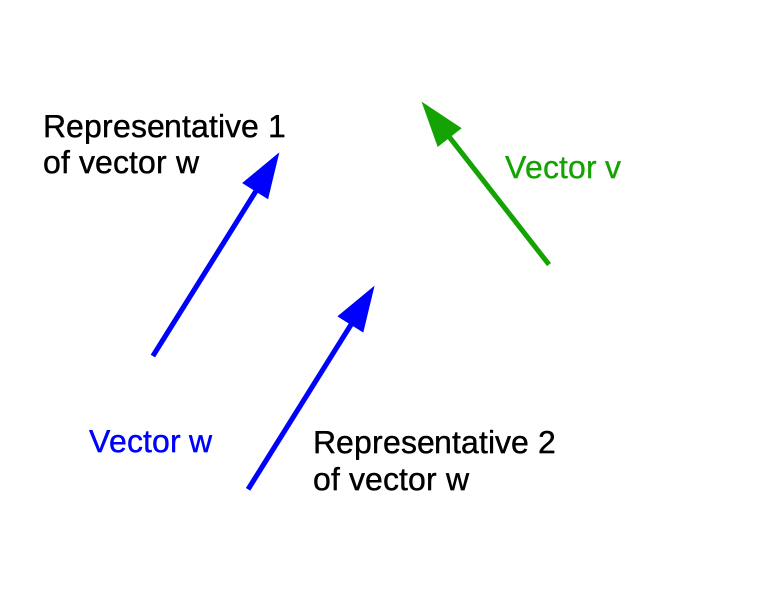
\includegraphics{odg/vector-physics-perspective.png}

\hypertarget{intro-linalg-computer-science-perspective}{%
\subsection{Computer Science Perspective}\label{intro-linalg-computer-science-perspective}}

In the computer science perspective vectors are ordered list of numbers. Later we will see that vectors can also contain more general objects like strings. As an example, we assume that we are analyzing carcasses and the only thing we know about a carcass is its slaughter-weight (SW) and its price (P). The different carcasses can then be represented by a pair of numbers the first being the slaughter-weight and the second being the price. It is important to note here, that the order of the number matters. In terms of vectors, here each carcass is represented by a two-dimensional vector.

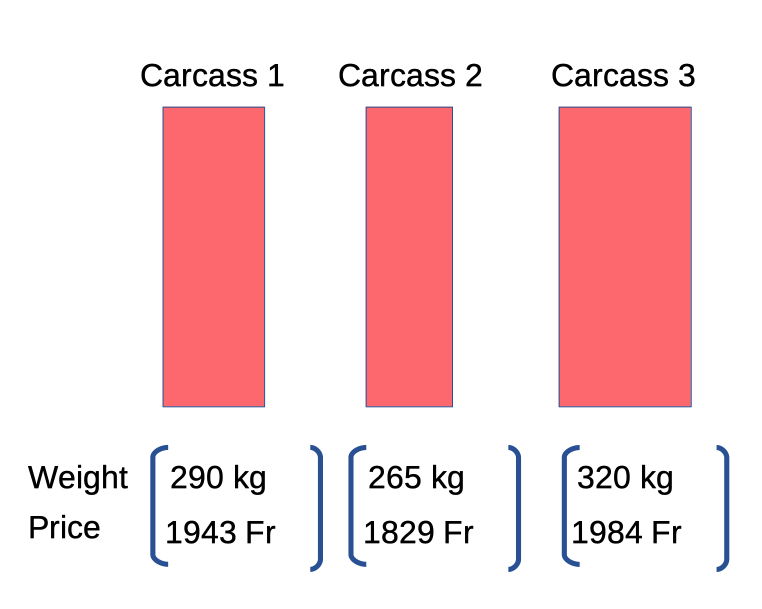
\includegraphics{odg/vector-cs-perspecitve.png}

\hypertarget{intro-linalg-geometric-context}{%
\subsection{Geometric Context}\label{intro-linalg-geometric-context}}

Some basic properties of vectors are introduced using the geometric context, that a vector is an arrow located in a certain coordinate system with its tail sitting at the origin of the coordinate system. This is a little bit different from the physics perspective (see \ref{intro-linalg-physics-perspective}) where the arrow can sit anywhere in space. In linear algebra it is almost always the case that vectors are rooted at the origin. Once we understand the properties of vectors in the context of arrows in space, we can then translate these properties to the list-of-numbers point of view (see \ref{intro-linalg-computer-science-perspective}) considering the coordinates of the vectors.

\hypertarget{intro-linalg-coordinate-system}{%
\subsection{Coordinate System}\label{intro-linalg-coordinate-system}}

It is important to introduce the coordinate system, because this will be the basis of the correspondence between the two perspectives of linear algebra. For the moment, we focus on two dimensions. The horizontal line is called the x-axis and the vertical line is called the y-axis. The place where the two lines intersect is called the origin. An arbitrary length is chosen to represent \(1\). The coordinates of a vector is a pair of numbers that give instructions for how to get from the tail of that vector at the origin to its tip. The first number tells you how far to walk along the x-axis (positive numbers indicating rightward motion, negative numbers indicating leftward motion) and the second number tell you how far to walk parallel to the y-axis (positive numbers indicating upward motion, negative numbers indicating downward motion).

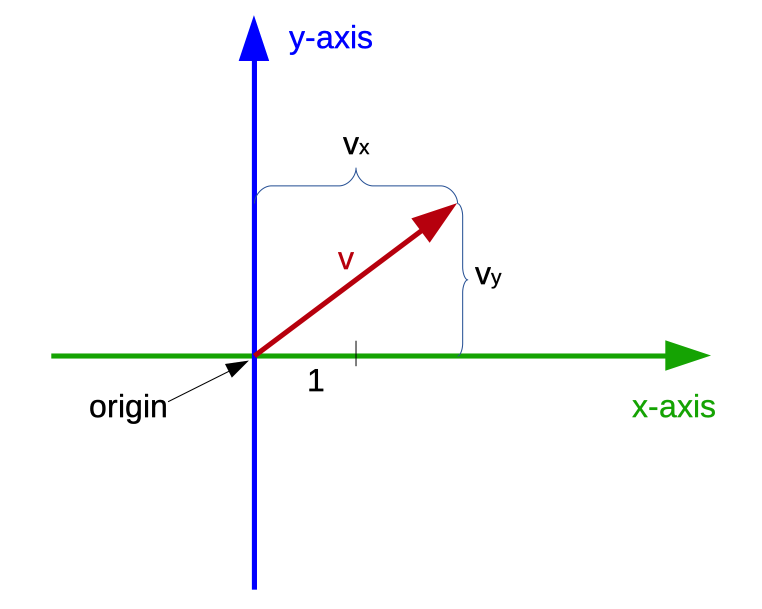
\includegraphics{odg/coordinate-system.png}

\hypertarget{intro-linalg-vector-operations}{%
\subsection{Vector Operations}\label{intro-linalg-vector-operations}}

The vectors by themselves can be pretty interesting objects, but they get really useful when considering some operations that we can perform on them. Here we consider three basic operations.

\begin{enumerate}
\def\labelenumi{\arabic{enumi}.}
\tightlist
\item
  addition
\item
  multiplication by a scalar number and
\item
  dot product
\end{enumerate}

\hypertarget{intro-linalg-vector-addition}{%
\subsubsection{Addition}\label{intro-linalg-vector-addition}}

Let us assume, we have two vectors \(v\) and \(w\). To add these two vectors, move the second one such that its tail sits at the tip of the first one. Then draw a new vector from the tail of the first one to the tip of the second one. The new vector corresponds to the sum of the two vectors (Figure \ref{fig:vector-sum}).

\begin{figure}
\centering
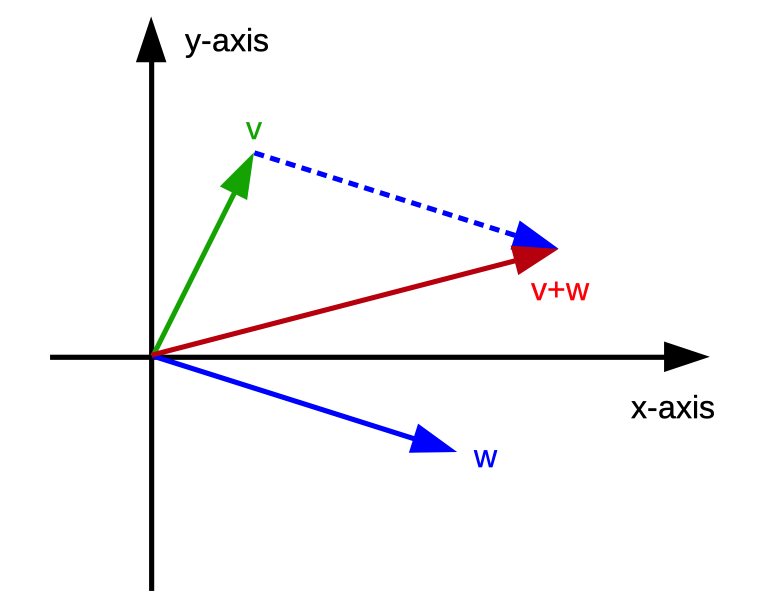
\includegraphics{odg/vector-sum.png}
\caption{\label{fig:vector-sum}Addition of two vectors}
\end{figure}

Numerically, vector addition corresponds to summing up each of the coordinates individually. Hence if we have two vectors \(v\) and \(w\) with their coordinates given as

\[v = \left[\begin{array}{c} v_x \\ v_y \end{array}\right] \text{, } w = \left[\begin{array}{c} w_x \\ w_y \end{array}\right]\]

then the sum \(v+w\) has coordinates

\[v+w =  \left[\begin{array}{c} v_x + w_x \\ v_y+w_y \end{array}\right]\]

\hypertarget{intro-linalg-vector-scalar-multiplication}{%
\subsubsection{Multiplication by a Scalar Number}\label{intro-linalg-vector-scalar-multiplication}}

This operation is best understood by looking at a few examples. If we take the number \(2\) and multiply it by a certain vector \(v\), this means that we stretch out the vector \(v\) such that it is \(2\) times as long as the original vector. Multiplication of a vector with positive numbers does not change the direction of the vector. Multiplying a vector \(v\) with a negative number like \(-0.5\) then the direction gets flipped around and then squished by \(0.5\).

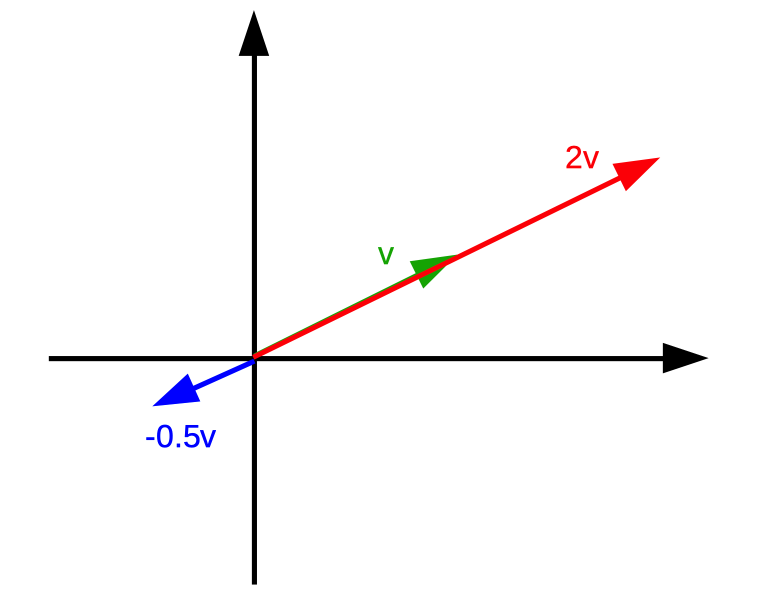
\includegraphics{odg/vector-scalar-multiplication.png}

The operation of multiplying a vector by a given number, like \(2\) or \(-0.5\) is also called \textbf{scaling} and that is the reason why in linear algebra the numbers like \(2\) and \(-0.5\) are called \textbf{scalar} numbers or just scalars. Numerically, stretching a vector by a given number like \(2\), corresponds to multiplying each of the coordinate components by that factor \(2\). For a vector \(v\) with coordinate components \(v_x\) and \(v_y\), the vector \(2v\) has coordinates \(2v_x\) and \(2v_y\)

\[v = \left[\begin{array}{c} v_x \\ v_y \end{array}\right] \text{, }\quad 2v = \left[\begin{array}{c} 2v_x \\ 2v_y \end{array}\right]\]

\hypertarget{intro-linalg-dot-product}{%
\subsubsection{Dot Product}\label{intro-linalg-dot-product}}

The dot product is explained in a different video that can be seen on \url{https://youtu.be/LyGKycYT2v0}. Numerically, if you have two vectors of the same dimension, meaning two lists of numbers of the same length, e.g. \(v\) and \(w\) then their dot product \(v \cdot w\) can be computed by pairing up all of the coordinates, multiplying these pairs together and adding the result. So the vectors

\[v = \left[\begin{array}{c} v_x \\ v_y \end{array}\right] \text{ and } w= \left[\begin{array}{c} w_x \\ w_y \end{array}\right]\]

their dot product \(v \cdot w\) then is computed as

\[v \cdot w = v_x * w_x + v_y * w_y\]

\hypertarget{intro-linalg-matrices}{%
\section{Matrices}\label{intro-linalg-matrices}}

The introduction to the topic of matrices is available from \url{https://youtu.be/kYB8IZa5AuE} and \url{https://youtu.be/XkY2DOUCWMU}. An \(m \times n\) matrix is a table-like object of \(m*n\) numbers arranged in \(m\) rows and \(n\) columns. In general the \(m \times n\) matrix \(A\) has the following structure.

\[
A = \left[
\begin{array}{cccc}
a_{11}  &  a_{12} &  \ldots  &  a_{1n} \\
a_{21}  &  a_{22} &  \ldots  &  a_{2n} \\
\vdots  &         &          &  \vdots \\
a_{m1}  &  a_{m2} &  \ldots  &  a_{mn}
\end{array}
\right]
\]

The \(m*n\) numbers inside of the square brackets are called elements of the matrix. The element of matrix \(A\) that is in row \(i\) and in column \(j\) is called \(a_{ij}\) or \((A)_{ij}\). As an example

\[
A =  \left[
\begin{array}{ccc}
2  &  3  &  1  \\
5  &  1  &  2
\end{array}
\right]
\]
is a \(2 \times 3\) matrix. In the first row the second element corresponds to \((A)_{12} = a_{12} = 3\). An \(n\times n\) matrix (i.e.~a matrix with equal numbers of rows and columns) is called a \textbf{quadratic} matrix. Two matrices \(A\) and \(B\) are called \textbf{equal}, if they have the same number of rows and columns and if the corresponding elements are the same, i.e.

\[
(A)_{ij} = (B)_{ij} \text{ for all i and j}
\]

\hypertarget{intro-linalg-special-matrices}{%
\subsection{Special Matrices}\label{intro-linalg-special-matrices}}

The following matrices are special and are used in special cases.

\begin{itemize}
\tightlist
\item
  \textbf{Nullmatrix}: The \(m\times n\) matrix \(0\) is called Nullmatrix, if each element is equal to zero.
\item
  \textbf{Upper Triangular Matrix}: The square matrix \(R\) is called upper triangular matrix, if \((R)_{ij} = 0\) for \(i>j\).
\item
  \textbf{Lower Triangular Matrix}: The square matrix \(L\) is called lower triangular matrix, if \((L)_{ij} = 0\) for \(i<j\).
\item
  \textbf{Diagonal Matrix}: The square matrix \(D\) is called diagonal matrix, if \((D)_{ij} = 0\) for \(i\ne j\).
\item
  \textbf{Identity Matrix}: The diagonal matrix \(I\) is called identity matrix, if all diagonal elements \((I)_{ii} = 1\).
\item
  \textbf{Column Vector}: A \(m\times 1\) matrix is often called a column vector.
\item
  \textbf{Row Vector}: A \(1\times n\) matrix is is often called a row vector.
\end{itemize}

\hypertarget{intro-linalg-matrix-operation}{%
\subsection{Matrix Operations}\label{intro-linalg-matrix-operation}}

The following operations with matrices are defined.

\hypertarget{intro-linalg-matrix-addition}{%
\subsubsection{Addition}\label{intro-linalg-matrix-addition}}

For two \(m\times n\) matrices \(A\) and \(B\), their sum \(A+B\) is again a \(m\times n\) matrix with each element corresponding to the sum of the corresponding elements from \(A\) and \(B\). Hence, we can write

\[(A+B)_{ij} = (A)_{ij} + (B)_{ij} \text{ for all i and j}\]

\hypertarget{intro-linalg-matrix-multiplication-with-number}{%
\subsubsection{Multiplication with a Number}\label{intro-linalg-matrix-multiplication-with-number}}

A \(m\times n\) matrix A is multiplied by a number \(\alpha\) by multiplying every element \((A)_{ij}\) of \(A\) with \(\alpha\). The result \(\alpha * A\) is computed as \((\alpha * A)_{ij} = \alpha * (A)_{ij}\) for all \(i\) and \(j\).

\hypertarget{intro-linalg-multiplication-two-matrices}{%
\subsubsection{Multiplication of two Matrices}\label{intro-linalg-multiplication-two-matrices}}

Given a \(m\times n\) matrix \(A\) and a \(n\times p\) matrix \(B\), their matrix product \(AB\) is a \(m\times p\) matrix with

\[ (AB)_{ij} = \sum_{k=1}^n (A)_{ik} * (B)_{kj} = (A)_{i1} * (B)_{1j} + (A)_{i2} * (B)_{2j} + \ldots + (A)_{in} * (B)_{nj}\]

\hypertarget{intro-linalg-laws-matrix-operations}{%
\subsubsection{Laws of Matrix Operations}\label{intro-linalg-laws-matrix-operations}}

\begin{itemize}
\tightlist
\item
  \textbf{Commutativity}: For two \(m\times n\) matrices \(A\) and \(B\) the addition is commutative, i.e. \(A + B = B + A\).
\item
  \textbf{Associativity of addition}: For \(m\times n\) matrices \(A\), \(B\) and \(C\), the addition is associative, i.e., \(A + (B + C) = (A + B) + C\)
\item
  \textbf{Associativity of multiplication}: For a \(m\times n\) matrix \(A\), a \(n \times p\) matrix \(B\) and a \(p \times q\) matrix \(C\), the multiplication is associative, i.e., \(A(BC) = (AB)C\)
\item
  \textbf{Distributivity}: For \(m\times n\) matrices \(A\) and \(B\) and \(n\times p\) matrices \(C\) and \(D\), the distributive law holds, i.e., \((A+B)C = AC + BC\) and \(A(C + D) = AC + AD\)
\end{itemize}

\hypertarget{intro-linalg-laws-matrix-transpose}{%
\subsubsection{Matrix Transpose}\label{intro-linalg-laws-matrix-transpose}}

Given a \(m\times n\) matrix \(A\), then the \(n\times m\) matrix \(A^T\) is called its \textbf{transpose}, if \((A^T)_{ij} = A_{ji}\). The matrix \(A\) is called \textbf{symmetric}, if \(A = A^T\). For every matrix \(A\) the transpose of the transpose is the matrix itself, i.e., \((A^T)^T = A\). For any \(m\times n\) matrices \(A\) and \(B\), the transpose \((A+B)^T\) of their sum \((A+B)\) is computed as

\[(A+B)^T = A^T + B^T\]

For every \(m\times n\) matrix \(A\) and every \(n\times p\) matrix \(B\), it holds that

\[(AB)^T = B^T A^T\]

\hypertarget{intro-linalg-inverse-matrix}{%
\subsubsection{Inverse of a Matrix}\label{intro-linalg-inverse-matrix}}

In this section, we are looking at square matrices. The \textbf{inverse} \(X\) of a square matrix \(A\) is defined as the square matrix that satisfies the condition \(AX = I\). If the inverse matrix \(X\) exists, then the matrix \(A\) is called invertable. If \(X\) does not exist, \(A\) is called singular. If the inverse of a matrix \(A\) exists, it is uniquely determined and we call it \(A^{-1}\).

Let us assume two invertable \(n\times n\) matrices \(A\) and \(B\), then the following equations hold

\begin{enumerate}
\def\labelenumi{\arabic{enumi}.}
\tightlist
\item
  \(A^{-1}A = I\)
\item
  \(A^{-1}\) is invertable and \((A^{-1})^{-1} = A\)
\item
  \(I\) is invertable and \(I^{-1} = I\)
\item
  \(AB\) is invertable and \((AB)^{-1} = B^{-1}A^{-1}\)
\item
  \(A^T\) is invertable and \((A^T)^{-1} = (A^{-1})^T\)
\end{enumerate}

For every square matrix \(A\), the following statements are equivalent.

\begin{enumerate}
\def\labelenumi{\arabic{enumi}.}
\tightlist
\item
  \(A\) is invertable
\item
  The system of equations \(Ax = b\) is solvable for every \(b\).
\item
  The system of equations \(Ax = 0\) has only the trivial solution \(x=0\).
\end{enumerate}

\hypertarget{intro-linalg-orthogonal-matrix}{%
\subsubsection{Orthogonal Matrices}\label{intro-linalg-orthogonal-matrix}}

A square matrix \(A\) is called \textbf{orthogonal}, if the condition \(A^TA = I\) holds. For two orthogonal matrices \(A\) and \(B\), the following statements hold.

\begin{enumerate}
\def\labelenumi{\arabic{enumi}.}
\tightlist
\item
  \(A\) is invertable and \(A^{-1} = A^T\)
\item
  \(A^{-1}\) is orthogonal
\item
  \(AB\) is orthogonal
\item
  \(I\) is orthogonal
\end{enumerate}

\hypertarget{intro-linalg-systems-of-equations}{%
\section{Systems Of Equations}\label{intro-linalg-systems-of-equations}}

Systems of linear equations are introduced based on \citep{Nipp2002} and \citep{Searle1971}. Solving systems of linear equations is one of the fundamental tasks of linear algebra. We start with a general example of a system of linear equations which is given as

\begin{align}
 x_1 + 2x_2 &= 5 \notag \\
2x_1 + 3x_2 &= 8
\label{eq:intro-linalg-first-example}
\end{align}

In \eqref{eq:intro-linalg-first-example} we are given a system of linear equations with two equations and two unknowns \(x_1\) and \(x_2\). The aim is to find numeric values for \(x_1\) and \(x_2\) such that both equations are satisfied. Inserting the values \(x_1 = 1\) and \(x_2 = 2\) into the above equations show that they are both satisfied. Hence the set \(L = \{x_1 = 1, x_2 = 2\}\) consisting of the values for \(x_1\) and \(x_2\) that satisfy both equations is called a solution or a solution set for the above shown equations.

In general, a linear system of equations consists of \(m\) equations and \(n\) unknowns. In the example \eqref{eq:intro-linalg-first-example}, \(m=2\) and \(n=2\).

The example in \eqref{eq:intro-linalg-no-solution} does not have any solutions.

\begin{align}
 x_1 +  x_2 &= 4 \notag \\
2x_1 + 2x_2 &= 5
\label{eq:intro-linalg-no-solution}
\end{align}

This can be seen, that if the first equation in \eqref{eq:intro-linalg-no-solution} is multiplied by \(2\), we get \(2x_1 + 2x_2 = 8\) which contradicts the second equation shown in \eqref{eq:intro-linalg-no-solution}.

A system with \(m=2\) equations and \(n=3\) unknowns in shown in \eqref{eq:intro-linalg-infnr-solution}.

\begin{align}
 x_1 -  x_2 +  x_3 &= 2 \notag \\
2x_1 +  x_2 -  x_3 &= 4  
\label{eq:intro-linalg-infnr-solution}
\end{align}

There are infinitely many solutions consisting of \(x_1 = 2\), \(x_2 = \alpha\) and \(x_3 = \alpha\) for any real number \(\alpha\).

The examples in \eqref{eq:intro-linalg-first-example}, \eqref{eq:intro-linalg-no-solution} and \eqref{eq:intro-linalg-infnr-solution} already show all possible cases that may occur when solving linear systems of equations. The question is how to determine the set of all solutions of a system of linear equations.

\hypertarget{intro-linalg-matrix-vector-notation}{%
\subsection{Matrix-Vector Notation}\label{intro-linalg-matrix-vector-notation}}

So far, we have written systems of linear equations explicitly in the sense that every equation was written on one line. For small systems this is not a problem. But when the number of equations (\(m\)) and the number of unknowns (\(n\)) get very large, the explicit notation is no longer feasible. Hence, we need a notation that can also be used for large systems of equations. The so-called matrix-vector notation provides an efficient way to write down large systems of equations very efficiently.

We return to the example given by \eqref{eq:intro-linalg-first-example} and we define the matrix \(A\) to be

\[
A = \left[
\begin{array}{cc}
1  &  2 \\
2  &  3
\end{array}
\right], 
\]

the vector \(x\) to be

\[
x = \left[
\begin{array}{c}
x_1  \\
x_2  
\end{array}
\right], 
\]

and the vector \(y\) to be

\[
y = \left[
\begin{array}{c}
5  \\
8  
\end{array}
\right], 
\]

With these definitions, we can write the system of equations given in \eqref{eq:intro-linalg-first-example} using matrix-vector notation as

\begin{equation}
A \cdot x = y
\label{eq:intro-linalg-matrix-vector-notation}
\end{equation}

\hypertarget{intro-linalg-solving-systems-of-linear-equations}{%
\section{Solving Systems of Linear Equations}\label{intro-linalg-solving-systems-of-linear-equations}}

If matrix \(A\) in \eqref{eq:intro-linalg-matrix-vector-notation} is not singular, i.e.~the inverse Matrix \(A^{-1}\) of \(A\) does exist, the solution \(x\) to \eqref{eq:intro-linalg-matrix-vector-notation} can be written as \(x = A^{-1}y\). This result is obtained by pre-multiplying both sides of \eqref{eq:intro-linalg-matrix-vector-notation} with \(A^{-1}\) and since a matrix times its inverse results in the identity matrix \(I\), the solution is obtained as

\begin{align}
            A \cdot x  &=  y \notag \\
A^{-1}\cdot A \cdot x  &=  A^{-1} \cdot y \notag \\
            I \cdot x  &=  A^{-1} \cdot y \notag \\
                    x  &=  A^{-1} \cdot y
\label{eq:intro-linalg-matrix-vector-notation-solution-derivation}
\end{align}

For systems of equations with a singular matrix \(A\), solutions can be found, if the equations are \textbf{consistent}. The linear equations \(Ax = y\) are consistent, if any linear relationship existing among the rows of \(A\) also exist among the corresponding elements of \(y\). As a simple example, the equations

\[
\left[
\begin{array}{cc}
1  &  2  \\
3  &  6
\end{array}\right]
\left[
\begin{array}{c}
x_1  \\
x_2
\end{array}\right]
=
\left[
\begin{array}{c}
7  \\
21
\end{array}\right]
\]
are consistent. In the matrix on the left the second row corresponds to three times the first row and in the vector on the right, the second element is also three times the first element. In contrast the equations

\[
\left[
\begin{array}{cc}
1  &  2  \\
3  &  6
\end{array}\right]
\left[
\begin{array}{c}
x_1  \\
x_2
\end{array}\right]
=
\left[
\begin{array}{c}
7  \\
24
\end{array}\right]
\]
are not consistent. From this example, we can already see that non-consistent equations do not have any solutions. But consistent equations \(Ax = y\) have a solution which can be written as \(x = Gy\) if and only if, \(AGA = A\) which means that \(G\) is a so-called generalized inverse of \(A\). The matrix \(G\) is often written as \(A^-\). The proof of this statement is given on page 9 of \citep{Searle1971}.

\hypertarget{quan-gen}{%
\chapter{Basics in Quantitative Genetics}\label{quan-gen}}

As already mentioned in section \ref{geno-pheno}, the central dogma of molecular biology tells us that the genotype is the basics of any phenotypic expression. The genotype of an individual is composed of a number of genes which are also called \textbf{loci}. In this section, we start with the simplest possible genetic architecture where the genotype is composed by just one locus. The connection between the genotype and the phenotype is modeled according to equation \eqref{eq:phengenenv}. The phenotype is assumed to be a quantitative trait. That means we are not looking at binary or categorical traits. Categorical traits can just take a limited number of different levels. Examples of categorical traits are the horn status in cattle or certain color characteristics. Quantitative traits do not take discrete levels but they show specific distributions.

\hypertarget{single-locus-quant-trait}{%
\section{Single Locus - Quantitative Trait}\label{single-locus-quant-trait}}

In Livestock there are not many examples where a quantitative trait is influenced by just one locus. But this case helps in understanding the foundation of more complex genetic architectures. We start by looking at the following idealized population (Figure \ref{fig:idealpopsingletrait}).

\begin{figure}
\centering
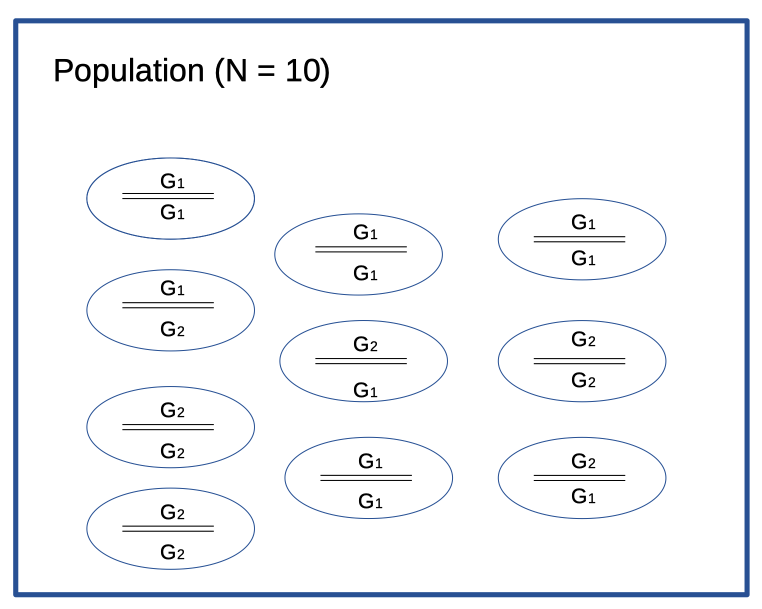
\includegraphics{odg/idealpopsingletrait.png}
\caption{\label{fig:idealpopsingletrait}Idealized Population With A Single Locus}
\end{figure}

\hypertarget{qg-terminology}{%
\subsection{Terminology}\label{qg-terminology}}

The different genetic variants that are present at our Locus \(G\) are called \textbf{alleles}. When looking at all individuals in the population for our locus, we have two different alleles \(G_1\) and \(G_2\). Hence, we call the locus \(G\) to be a \textbf{bi-allelic} locus. In any given individual of the population, the two alleles of the locus \(G\) together are called the individuals \textbf{genotype}. All possible combinations of the two alleles at the locus \(G\) leads to a total number of three genotypes. It is important to mention that the order of the alleles in a given genotype is not important. Hence, \(G_1G_2\) and \(G_2G_1\) are the same genotype. The two genotypes \(G_1G_1\) and \(G_2G_2\) are called \textbf{homozygous} and the genotype \(G_1G_2\) is called \textbf{heterozygous}.

\hypertarget{qg-frequency}{%
\section{Frequencies}\label{qg-frequency}}

To be able to characterize our population with respect to the locus of interest, we are first looking at some frequencies. These are measures of how often a certain allele or genotype does occur in our population. For our example population shown in Figure \ref{fig:idealpopsingletrait}, the \textbf{genotype frequencies} are

\begin{align}
f(G_1G_1) &= \frac{4}{10} = 0.4 \notag \\
f(G_1G_2) &= \frac{3}{10} = 0.3 \notag \\
f(G_2G_2) &= \frac{3}{10} = 0.3  \label{eq:genotypefreq}
\end{align}

The \textbf{allele frequencies} can be determined either by counting or they can be computed from the genotype frequencies.

\begin{align}
f(G_1) &= f(G_1G_1) + {1\over 2}*f(G_1G_2) = 0.55 \notag \\
f(G_2) &= f(G_2G_2) + {1\over 2}*f(G_1G_2) = 0.45 \label{eq:allelefreq}
\end{align}

\hypertarget{hw-eq}{%
\section{Hardy-Weinberg Equilibrium}\label{hw-eq}}

The Hardy-Weinberg equilibrium is the central law of how allele frequencies and genotype frequencies are related in an idealized population. Given the allele frequencies

\begin{align}
f(G_1) &= p \notag \\
f(G_2) &= q = 1-p
\label{eq:allelefreq}
\end{align}

During mating, we assume that in an idealized population alleles are combined independently. This leads to the genotype frequencies shown in Table \ref{tab:tabgenfreq}.

\begin{table}

\caption{\label{tab:tabgenfreq}Genotype Frequencies under Hardy-Weinberg equilibrium}
\centering
\begin{tabular}[t]{ccc}
\toprule
Alleles & $G_1$ & $G_2$\\
\midrule
$G_1$ & $f(G_1G_1) = p^2$ & $f(G_1G_2) = p*q$\\
$G_2$ & $f(G_1G_2) = p*q$ & $f(G_2G_2) = q^2$\\
\bottomrule
\end{tabular}
\end{table}

Summing up the heterozygous frequencies leads to

\begin{align}
f(G_1G_1) &= p^2 \notag \\
f(G_1G_2) &= 2pq \notag \\
f(G_2G_2) &= q^2
\label{eq:genofreq}
\end{align}

Comparing these expected genotype frequencies in a idealized population under the Hardy-Weinberg equilibrium to what we found for the small example population in Figure \ref{fig:idealpopsingletrait}, we can clearly say that the small example population is not in Hardy-Weinberg equilibrium.

\hypertarget{value-mean}{%
\section{Value and Mean}\label{value-mean}}

Our goal is still to improve our population at the genetic level. The term improvement implies the need for a quantitative assessment of our trait of interest. Furthermore, we have to be able to associate the genotypes in the population to the quantitative values of our trait.

\hypertarget{geno-value}{%
\subsection{Genotypic Values}\label{geno-value}}

The values \(V_{ij}\) to each genotype \(G_iG_j\) are assigned as shown in Figure \ref{fig:genotypicvalue}.

\begin{figure}
\centering
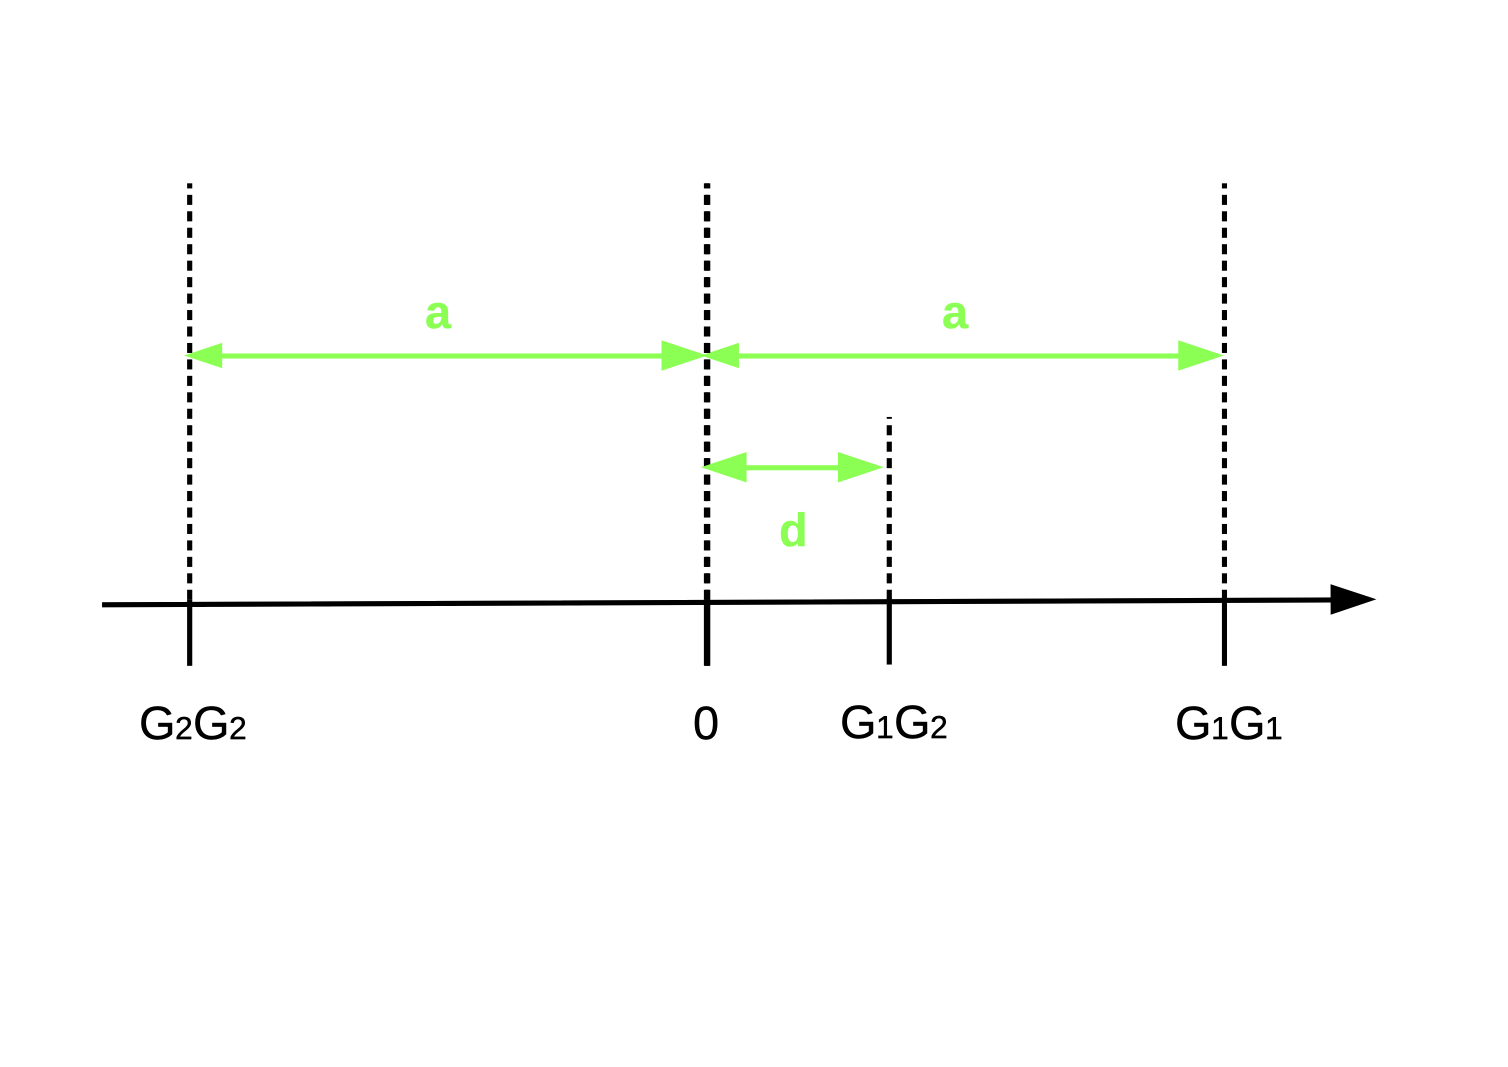
\includegraphics{odg/genotypicvalue.png}
\caption{\label{fig:genotypicvalue}Genotypic Values}
\end{figure}

The origin of the genotypic values is placed in the middle between the two homozygous genotypes \(G_2G_2\) and \(G_1G_1\). Here we are assuming that \(G_1\) is the favorable allele. This leads to values of \(+a\) for genotype \(G_1G_1\) and of \(-a\) for genotype \(G_2G_2\). The value of genotype \(G_1G_2\) is set to \(d\) and is called dominance deviation. Table \ref{tab:tabsumgenvalue} summarizes the values for all genotypes.

\begin{table}

\caption{\label{tab:tabsumgenvalue}Values for all Genotypes}
\centering
\begin{tabular}[t]{ccc}
\toprule
Variable & Genotype & Values\\
\midrule
$V_{11}$ & $G_1G_1$ & a\\
$V_{12}$ & $G_1G_2$ & d\\
$V_{22}$ & $G_2G_2$ & -a\\
\bottomrule
\end{tabular}
\end{table}

\hypertarget{pop-mean}{%
\subsection{Population Mean}\label{pop-mean}}

For the complete population, we can compute the \textbf{population mean} (\(\mu\)) of all values at the locus \(G\). This mean corresponds to the expected value and is computed as

\begin{align}
\mu &= V_{11} * f(G_1G_1) + V_{12} * f(G_1G_2) + V_{22} * f(G_2G_2) \notag \\
    &= a * p^2 + d *2pq + (-a) * q^2 \notag \\
    &= (p-q)a + 2pqd
\label{eq:popmean}
\end{align}

The population mean depends on the values \(a\) and \(d\) and on the allele frequencies \(p\) and \(q\). The larger the difference between \(p\) and \(q\) the more influence the value \(a\) has in \(\mu\), because for very different \(p\) and \(q\) the product \(2pq\) is very small. On the other hand, if \(p=q=0.5\), then \(\mu = 0.5d\). For loci with \(d=0\), the population mean \(\mu = (p-q)a\) and hence, if in addition we have \(p=q\), then \(\mu=0\).

\hypertarget{breed-value}{%
\subsection{Breeding Values}\label{breed-value}}

The term \textbf{breeding value} is defined as shown in Definition \ref{def:defbreedingvalue}.

\BeginKnitrBlock{definition}[Breeding Value]
\protect\hypertarget{def:defbreedingvalue}{}{\label{def:defbreedingvalue} \iffalse (Breeding Value) \fi{} }The breeding value of an animal \(i\) is defined as two times the difference between the mean value of offsprings of animal \(i\) and the population mean.
\EndKnitrBlock{definition}

Applying this definition and using the parameters that we have computed so far leads to the following formulas for the breeding value of an animal with a certain genotype.

\hypertarget{breeding-value-for-g_1g_1}{%
\subsubsection{\texorpdfstring{Breeding value for \(G_1G_1\)}{Breeding value for G\_1G\_1}}\label{breeding-value-for-g_1g_1}}

Assume that we have a given parent \(S\) with a genotype \(G_1G_1\) and we want to compute its breeding value. Let us further suppose that our single parent \(S\) is mated to a potentially infinite number of animals from the idealized population, then we can deduce the following mean genotypic value for the offspring of parent \(S\).

\vspace{5ex}

\begin{tabular}{|c|c|c|}
\hline
& \multicolumn{2}{|c|}{Mates of $S$} \\
\hline
& $f(G_1) = p$       &  $f(G_2) = q$   \\
\hline
Parent $S$       &                    &                 \\
\hline
$f(G_1) = 1$ &  $f(G_1G_1) = p$   &  $f(G_1G_2) = q$\\
\hline
\end{tabular}

\vspace{5ex}

Because parent \(S\) has genotype \(G_1G_1\), the frequency \(f(G_1)\) of a \(G_1\) allele coming from \(S\) is \(1\) and the frequency \(f(G_2)\) of a \(G_2\) allele is 0. The expected genetic value (\(\mu_{11}\)) of the offspring of animal \(S\) can be computed as

\begin{equation}
\mu_{11} = p*a + q*d
\label{eq:MeanOffGen11}
\end{equation}

Applying definition \ref{def:defbreedingvalue}, we can compute the breeding value (\(BV_{11}\)) for animal \(S\) as shown in equation \eqref{eq:BVGen11} while using the results given by equations \eqref{eq:MeanOffGen11} and \eqref{eq:popmean}.

\begin{align}
BV_{11} &=  2*(\mu_{11} - \mu)  \notag \\
        &=  2\left(pa + qd - \left[(p - q)a + 2pqd \right] \right) \notag\\
        &=  2\left(pa + qd - (p - q)a - 2pqd \right) \notag\\
        &=  2\left(qd + qa - 2pqd\right) \notag \\
        &=  2\left(qa + qd(1 - 2p)\right) \notag \\
        &=  2q\left(a + d(1 - 2p)\right) \notag \\
        &=  2q\left(a + (q-p)d\right)
\label{eq:BVGen11}
\end{align}

Breeding values for parents with genotypes \(G_2G_2\) and \(G_1G_2\) are derived analogously.

\hypertarget{breeding-value-for-g_2g_2}{%
\subsubsection{\texorpdfstring{Breeding value for \(G_2G_2\)}{Breeding value for G\_2G\_2}}\label{breeding-value-for-g_2g_2}}

First, we determine the expected genotypic value for offsprings of a parent \(S\) with genotype \(G_2G_2\)

\vspace{5ex}

\begin{tabular}{|c|c|c|}
\hline
& \multicolumn{2}{|c|}{Mates of parent $S$} \\
\hline
& $f(G_1) = p$       &  $f(G_2) = q$   \\
\hline
Parent $S$       &                    &                 \\
\hline
$f(G_2) = 1$ &  $f(G_1G_2) = p$   &  $f(G_2G_2) = q$\\
\hline
\end{tabular}

\vspace{5ex}

The expected genetic value (\(\mu_{22}\)) of the offspring of animal \(S\) can be computed as

\begin{equation}
\mu_{22} = pd - qa
\label{eq:MeanOffGen22}
\end{equation}

The breeding value \(BV_{22}\) corresponds to

\begin{align}
BV_{22} &=   2*(\mu_{22} - \mu)  \notag \\
        &=   2\left(pd - qa - \left[(p - q)a + 2pqd \right] \right) \notag \\
        &=   2\left(pd - qa - (p - q)a - 2pqd \right) \notag \\
        &=   2\left(pd - pa - 2pqd\right) \notag \\
        &=   2\left(-pa + p(1-2q)d\right) \notag \\
        &=  -2p\left(a + (q - p)d\right)
\label{eq:BVGen22}
\end{align}

\hypertarget{breeding-value-for-g_1g_2}{%
\subsubsection{\texorpdfstring{Breeding value for \(G_1G_2\)}{Breeding value for G\_1G\_2}}\label{breeding-value-for-g_1g_2}}

The genotype frequencies of the offsprings of a parent \(S\) with a genotype \(G_1G_2\) is determined in the following table.

\vspace{5ex}

\begin{tabular}{|c|c|c|}
\hline
& \multicolumn{2}{|c|}{Mates of parent $S$} \\
\hline
& $f(G_1) = p$       &  $f(G_2) = q$   \\
\hline
Parent $S$       &                    &                 \\
\hline
$f(G_1) = 0.5$ &  $f(G_1G_1) = 0.5p$   &  $f(G_1G_2) = 0.5q$\\
\hline
$f(G_2) = 0.5$ &  $f(G_1G_2) = 0.5p$   &  $f(G_2G_2) = 0.5q$\\
\hline
\end{tabular}

\vspace{5ex}

The expected mean genotypic value of the offsprings of parent \(S\) with genotype \(G_1G_2\) is computed as

\begin{equation}
\mu_{12} = 0.5pa + 0.5d - 0.5qa = 0.5\left[(p-q)a + d \right]
\label{eq:MeanOffGen12}
\end{equation}

The breeding value \(BV_{12}\) corresponds to

\begin{align}
ZW_{12} &=   2*(\mu_{12} - \mu) \notag \\
        &=   2\left(0.5(p-q)a + 0.5d - \left[(p - q)a + 2pqd \right] \right) \notag \\
        &=   2\left(0.5pa - 0.5qa + 0.5d - pa + qa - 2pqd \right) \notag \\
        &=   2\left(0.5(q-p)a + (0.5 - 2pq)d \right) \notag \\
        &=   (q-p)a + (1-4pq)d  \notag \\
        &=   (q-p)a + (p^2 + 2pq + q^2 -4pq)d  \notag \\
        &=   (q-p)a + (p^2 - 2pq + q^2)d  \notag \\
        &=   (q-p)a + (q - p)^2d   \notag \\
        &=   (q-p)\left[a + (q-p)d \right]
\label{eq:BVGen12}
\end{align}

\hypertarget{summary-of-breeding-values}{%
\subsubsection{Summary of Breeding Values}\label{summary-of-breeding-values}}

The term \(a + (q-p)d\) appears in all three breeding values. We replace this term by \(\alpha\) and summarize the results in the following table.

\begin{tabular}{|c|c|}
  \hline
  Genotype  &  Breeding Value\\
  \hline
  $G_1G_1$  &  $2q\alpha$    \\
  \hline
  $G_1G_2$  &  $(q-p)\alpha$ \\
  \hline
  $G_2G_2$  &  $-2p\alpha$   \\
  \hline
  \end{tabular}

\hypertarget{allele-substitution}{%
\subsection{Allele Substitution}\label{allele-substitution}}

Comparing the genotype \(G_2G_2\) with the genotype \(G_1G2\), one of the differences is in the number of \(G_1\)-alleles. \(G_2G_2\) has zero \(G_1\)-alleles and \(G_1G_2\) has one \(G_1\)-allele. They also have different breeding values. Because the breeding values are to be used to assess the value of a given genotype, any difference between the breeding values \(BV_{12}\) and \(B_{22}\) can be associated to that additional \(G_1\) allele in \(G_1G_2\) compared to \(G_2G_2\).

The computation of the difference between the breeding value \(BV_{12}\) and \(B_{22}\) results in

\begin{align}
    BV{12} - BV_{22} &=   (q-p)\alpha - \left( -2p\alpha \right)  \notag \\
                      &=   (q-p)\alpha + 2p\alpha \notag \\
                      &=   (q-p+2p)\alpha \notag \\
                      &=   (q+p)\alpha \notag \\
                      &=   \alpha
  \label{eq:AdditiveBv1}
\end{align}

The analogous computation can be done by comparing the breeding values \(BV_{11}\) and \(BV_{12}\).

\begin{align}
    BV_{11} - BV_{12} & = & 2q\alpha - (q-p)\alpha \notag \\
                      & = & \left(2q - (q-p)\right)\alpha \notag\\
                      & = & \alpha 
  \label{eq:AdditiveBv2}
\end{align}

The breeding values themselves depend on the allele frequencies. But the differences between breeding values are linear while replacing \(G_2\) alleles by \(G_1\) alleles. This replacement is also called allele-substitution and the term \(alpha\) is called \textbf{allele-substitution effect}.

\hypertarget{dominance-deviation}{%
\subsection{Dominance Deviation}\label{dominance-deviation}}

When looking at the difference between the genotypic value \(V_{ij}\) and the breeding value \(BV_{ij}\) for each of the three genotypes, we get the following results.

\begin{align}
  V_{11} - BV_{11} &=   a - 2q \alpha \notag \\
                   &=   a - 2q \left[ a + (q-p)d \right] \notag \\
                   &=   a - 2qa -2q(q-p)d \notag \\
                   &=   a(1-2q) - 2q^2d + 2pqd \notag \\
                   &=   \left[(p - q)a + 2pqd\right] - 2q^2d \notag \\
                   &=   \mu + D_{11} 
  \end{align}

\begin{align}
  V_{12} - BV{12} &=   d - (q-p)\alpha \notag \\
                   &=   d - (q-p)\left[ a + (q-p)d \right] \notag \\
                   &=   \left[(p-q)a + 2pqd\right] + 2pqd \notag \\
                   &=   \mu + D_{12}
  \end{align}

\begin{align}
  V_{22} - BV_{22} &=   -a - (-2p\alpha) \notag \\
                   &=   -a + 2p\left[ a + (q-p)d \right] \notag \\
                   &=   \left[(p-q)a + 2pqd\right] - 2p^2d \notag \\
                   &=   \mu + D_{22} \notag
  \end{align}

The difference all contain the population mean \(\mu\) plus a certain deviation. This deviation term is called \textbf{dominance deviation}.

\hypertarget{summary-of-values}{%
\subsection{Summary of Values}\label{summary-of-values}}

The following table summarizes all genotypic values all breeding values and the dominance deviations.

\begin{tabular}{|c|c|c|c|}
   \hline
   Genotyp  &  genotypic value     &  Breeding Value    &  Dominance Deviation \\
   $G_iG_j$ &  $V_{ij}$            &  $BV_{ij}$         &  $D_{ij}$           \\
   \hline
   $G_1G_1$ &  $a$                 &  $2q\alpha$        &  $-2q^2d$          \\
   \hline
   $G_1G_2$ &  $d$                 &  $(q-p)\alpha$     & $2pqd$             \\
   \hline
   $G_2G_2$ &  $-a$                &  $-2p\alpha$       & $-2p^2d$           \\
   \hline
\end{tabular}

The formulas in the above shown table assume that \(G_1\) is the favorable allele with frequency \(f(G_1) = p\). The allele frequency of \(G_2\) is \(f(G_2) = q\). Since we have a bi-allelic locus \(p+q=1\).

Based on the definition of dominance deviation, the genotypic values \(V_{ij}\) can be decomposed into the components population mean (\(\mu\)), breeding value (\(BV_{ij}\)) and dominance deviation (\(D_{ij}\)) according to equation \eqref{eq:SeparationGenoValue}.

\begin{align}
V_{ij} &=   \mu + BV_{ij} + D_{ij}
\label{eq:SeparationGenoValue}
\end{align}

Taking expected values on both sides of equation \eqref{eq:SeparationGenoValue} and knowing that the population mean \(\mu\) was defined as the expected value of the genotypic values in the population, i.e. \(E\left[ V \right] = \mu\), it follows that the expected values of both the breeding values and the dominance deviations must be \(0\). More formally, we have

\begin{align}
E\left[ V \right] &=  E\left[ \mu + BV + D \right] \notag \\
                  &=  E\left[ \mu \right]  + E\left[ BV \right] + E\left[ D \right] \notag \\
                  &=  \mu
\label{eq:ExpValueGenBvDom}
\end{align}

From the last line in equation \eqref{eq:ExpValueGenBvDom}, it follows that \(E\left[ BV \right] = E\left[ D \right] = 0\). This also shows that both breeding values and dominance deviations are defined as deviation from a given mean.

\hypertarget{variances}{%
\section{Variances}\label{variances}}

The population mean \(\mu\) and derived from that the breeding values were defined as expected values. Their main purpose is to assess the state of a given population with respect to a certain genetic locus and its effect on a phenotypic trait of interest. One of our primary goals in livestock breeding is to improve the populations at the genetic level through the means of selection and mating. Selection of potential parents that produce offspring that are closer to our breeding goals is only possible, if the selection candidates show a certain level of variation in the traits that we are interested in. In populations where there is no variation which means that all individuals are exactly at the same level, it is not possible to select potential parents for the next generation.

In statistics the measure that is most often used to assess variation in a certain population is called \textbf{variance}. For any given discrete random variable \(X\) the variance is defined as the second central moment of \(X\) which is computed as shown in equation \eqref{eq:VarianceDiscreteRV}.

\begin{equation}
Var\left[X\right] = \sum_{x_i \in \mathcal{X}} (x_i - \mu_X)^2 * f(x_i)
\label{eq:VarianceDiscreteRV}
\end{equation}

\vspace*{1ex}

\begin{tabular}{p{1cm}p{1cm}p{6cm}}
  where & $\mathcal{X}$: &  set of all possible $x$-values\\
        & $f(x_i)$       &  probability that $x$ assumes the value of $x_i$ \\
        & $\mu_X $       &  expected value $E\left[X\right]$ of $X$
  \end{tabular}

\vspace*{2ex}

In this section we will be focusing on separating the obtained variances into different components according to their causative sources. Applying the definition of variance given in equation \eqref{eq:VarianceDiscreteRV} to the genotypic values \(V_{ij}\), we obtain the following expression.

\begin{align}
\sigma_G^2 = Var\left[V\right] &=   (V_{11} - \mu)^2 * f(G_1G_1) \notag \\
                               &  +\  (V_{12} - \mu)^2 * f(G_1G_2) \notag \\
                               &  +\  (V_{22} - \mu)^2 * f(G_2G_2)
\label{eq:VarianceGenotypicValue}
\end{align}

where \(\mu = (p - q)a + 2pqd\) the population mean.

Based on the decomposition of the genotypic value \(V_{ij}\) given in \eqref{eq:SeparationGenoValue}, the difference between \(V_{ij}\) and \(\mu\) can be written as the sum of the breeding value and the dominance deviation. Then \(\sigma_G^2\) can be written as

\begin{align}
\sigma_G^2 = Var\left[V\right] &=   (BV_{11} + D_{11})^2 * f(G_1G_1) \notag \\
                               &  +\  (BV_{12} + D_{12})^2 * f(G_1G_2) \notag \\
                               &  +\  (BV_{22} + D_{22})^2 * f(G_2G_2)
\label{eq:GeneticVarianceBVDom}
\end{align}

Inserting the expressions for the breeding values \(BV_{ij}\) and for the dominance deviation \(D_{ij}\) found earlier and simplifying the equation leads to the result in \eqref{eq:FinalGeneticVariance}. A more detailed derivation of \(\sigma_G^2\) is given in the appendix (\ref{appendix-derivations}) of this chapter.

\begin{align}
  \sigma_G^2 &=  2pq\alpha^2 + \left(2pqd \right)^2 \notag\\
             &=  \sigma_A^2 + \sigma_D^2
\label{eq:FinalGeneticVariance}             
\end{align}

The formula in equation \eqref{eq:FinalGeneticVariance} shows that \(\sigma_G^2\) consists of two components. The first component \(\sigma_A^2\) is called the \textbf{genetic additive variance} and the second component \(\sigma_D^2\) is termed \textbf{dominance variance}. As shown in equation \eqref{eq:VarBV} \(\sigma_A^2\) corresponds to the variance of the breeding values. Because we have already seen that the breeding values are additive in the number of favorable alleles, \(\sigma_A^2\) is called genetic additive variance. Because \(\sigma_D^2\) corresponds to the variance of the dominance deviation effects (see equation \eqref{eq:VarDom}) it is called dominance variance.

\hypertarget{extension-to-more-loci}{%
\section{Extension To More Loci}\label{extension-to-more-loci}}

When only a single locus is considered, the genotypic values (\(V_{ij}\)) can be decomposed according to equation \eqref{eq:SeparationGenoValue} into population mean, breeding value and dominance deviation. When a genotype refers to more than one locus, the genotypic value may contain an additional deviation caused by non-additive combination effects.

\hypertarget{epistatic-interaction}{%
\subsection{Epistatic Interaction}\label{epistatic-interaction}}

Let \(V_A\) be the genotypic value of locus \(A\) and \(V_B\) denote the genotypic value of a second locus \(B\), then the total aggregate genotypic value \(V\) attributed to both loci \(A\) and \(B\) can be written as

\begin{equation}
V = V_A + V_B + I_{AB}
\label{eq:AggregateGenotypicValueTwoLoci}
\end{equation}

where \(I_{AB}\) is the deviation from additive combination of these genotypic values. When computing the population mean earlier in this chapter, we assumed that \(I\) was zero for all combinations of genotypes. If \(I\) is not zero for any combination of genes at different loci, those genes are said to \textbf{interact} with each other or to exhibit \textbf{epistasis}. The deviation \(I\) is called interaction deviation or epistatic deviation. If \(I\) is zero, the genes are called to act additively between loci. Hence \emph{additive action} may mean different things. When referring to one locus, it means absence of dominance. When referring to different loci, it means absence of epistasis.

Interaction between loci may occur between pairs or between higher numbers of different loci. The complex nature of higher order interactions, i.e., interactions between higher number of loci does not need to concern us. Because in the aggregate genotypic value \(V\), interaction deviations of all sorts are treated together in an overall interaction deviation \(I\). This leads to the following generalized form of decomposing the overall aggregate genotype \(V\) for the case of multiple loci affecting a certain trait of interest.

\begin{equation}
V = \mu + U + D + I
\label{eq:AggregateGenotypicValueMultipleLoci}
\end{equation}

where \(U\) is the sum of the breeding values attributable to the separate loci and \(D\) is the sum of all dominance deviations. For our purposes in livestock breeding where we want to assess the genetic potential of a selection candidate to be a parent of offspring forming the next generation, the \textbf{breeding value} is the most important quantity. The breeding value is of primary importance because a given parent passes a random sample of its alleles to its offspring. We have seen in section \ref{allele-substitution} that breeding values are additive in the number of favorable alleles. Hence the more favorable alleles a given parent passes to its offspring the higher the breeding value of this parent.

On the other hand, the dominance deviation measures the effect of a certain genotype occurring in an individual and the interaction deviation estimates the effects of combining different genotypes at different loci in the genome. But because parents do not pass complete genotypes nor do they pass stretches of DNA with several loci, but only a random collection of its alleles, it is really the breeding value that is of primary importance in assessing the genetic potential of a given selection candidate.

\hypertarget{interaction-variance}{%
\subsection{Interaction Variance}\label{interaction-variance}}

If genotypes at different loci show epistatic interaction effects as described in section \ref{epistatic-interaction}, the interactions give rise to an additional variance component called \(V_I\), which is the variance of interaction deviations. This new variance component \(V_I\) can be further decomposed into sub-components. The first level of sub-components is according to the number of loci that are considered. Two-way interactions involve two loci, three-way interactions consider three loci and in general \(n\)-way interactions arise from \(n\) different loci. The next level of subdivision is according to whether they include additive effects, dominance deviations or both.

In general it can be said that for practical purposes, interaction effects explain only a very small amount of the overall variation. As already mentioned in section @ref(\#epistatic-interaction) for livestock breeding, we are mostly interested in the additive effects. This is also true when looking at the variance components. Hence dominance variance and variances of interaction deviations are not used very often in practical livestock breeding application.

\hypertarget{genetic-models}{%
\section{Genetic Models}\label{genetic-models}}

In this chapter, we have seen how to model the genetic basis of a quantitative trait when a single locus affects the trait of interest. We call this a single-locus model. When several loci have an effect on a certain trait, then we talk about a \textbf{polygenic model}. Letting the number of loci affecting a certain phenotype tend to infinity, the resulting model is called \textbf{infinitesimal model}.

From a statistical point of view, the breeding values in an infinitesimal model are considered as a random effect with a known distribution. Due to the central limit theorem, this distribution is assumed to be a normal distribution. The central limit theorem says that the distribution of any sum of a large number of very small effects converges to a normal distribution. For our case where a given trait of interest is thought to be influenced by a large number of genetic loci each having a small effect, the sum of the breeding values of all loci together can be approximated by a normal distribution. Figure (\ref{fig:hist-clt}) shows the distribution for a sum of 10, 100 and 1000 components each. The histograms show a better approximation to the normal distribution the larger the number of components considered in the sum.

\begin{figure}
\centering
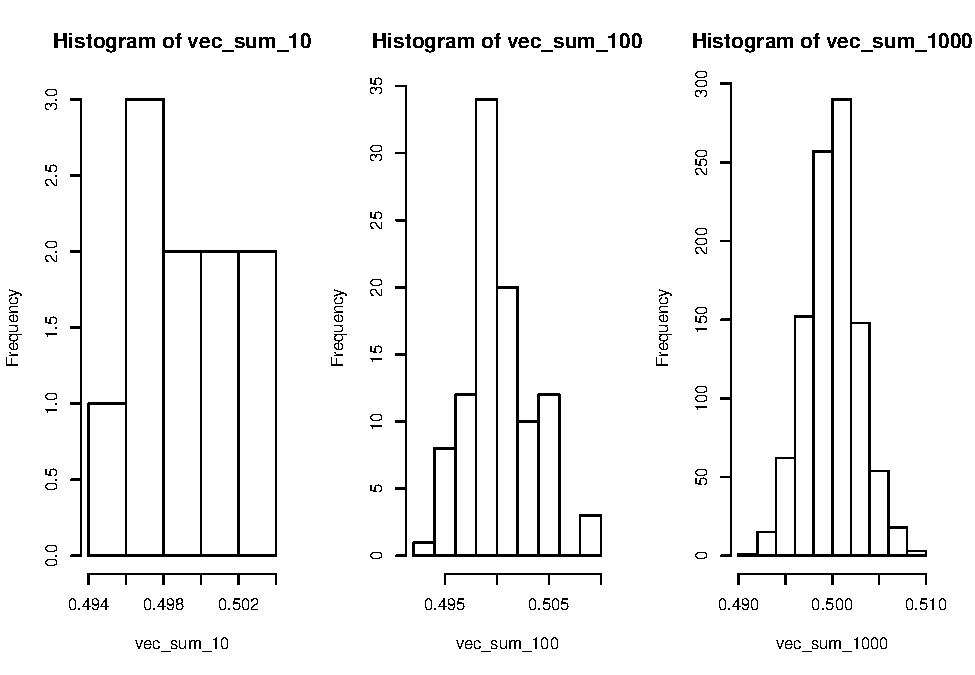
\includegraphics{bookdown-asmas-ss2020_files/figure-latex/hist-clt-1.pdf}
\caption{\label{fig:hist-clt}Distribution of Sums of Different Numbers of Components}
\end{figure}

\hypertarget{model-usage-in-routine-evaluations}{%
\subsection{Model Usage In Routine Evaluations}\label{model-usage-in-routine-evaluations}}

Traditional prediction of breeding values before the introduction of genomic selection is based on the infinitesimal model. When genomic selection was introduced which takes into account the information from a large number of loci, genomic breeding values are estimated using a polygenic model.

\hypertarget{appendix-derivations}{%
\section{Appendix: Derivations}\label{appendix-derivations}}

This section shows how the genetic variance in equation \eqref{eq:FinalGeneticVariance} is computed.

\begin{align}
\sigma_G^2  &=   (BV_{11} + D_{11})^2 * p^2                                       \notag \\
            &   +\  (BV_{12} + D_{12})^2 * 2pq                                    \notag \\
            &   +\  (BV_{22} + D_{22})^2 * q^2                                    \notag \\
            &=      \left(2q\alpha - 2q^2d   \right)^2 * p^2                      \notag \\
            &   +\  \left((q-p)\alpha + 2pqd \right)^2 * 2pq                      \notag \\
            &   +\  \left(-2p\alpha - 2p^2d  \right)^2 * q^2                      \notag \\
            &=      \left(4q^2\alpha^2 - 8q^3d\alpha + 4q^4d^2  \right) * p^2     \notag \\
            &   +\  \left(q^2\alpha^2 - 2pq\alpha^2 + p^2\alpha^2
                           - 4(q-p)pqd\alpha + 4p^2q^2d^2\right) * 2pq            \notag \\
            &   +\  \left(4p^2\alpha^2 + 8p^3d\alpha + 4p^4\alpha^2 \right) * q^2 \notag \\
            &=      4p^2q^2\alpha^2 - 8p^2q^3d\alpha + 4p^2q^4d^2                 \notag \\
            &   +\  2pq^3\alpha^2 - 4p^2q^2\alpha^2+ 2p^3q\alpha^2                \notag \\
            &   -\  8p^3q^2d\alpha + 8p^2q^3d\alpha + 8p^3q^3d^2                  \notag \\
            &   +\  4p^2q^2\alpha^2 + 8p^3q^2d\alpha + 4p^4q^2d^2                 \notag \\
            &=      4p^2q^2\alpha^2 + 4p^2q^4d^2                                  \notag \\
            &   +\  2pq^3\alpha^2 + 2p^3q\alpha^2                                 \notag \\
            &   +\  8p^3q^3d^2                                                    \notag \\
            &   +\  4p^4q^2d^2                                                    \notag \\
            &=      2pq\alpha^2 \left(p^2 + 2pq + q^2 \right)                     \notag \\
            &   +\  \left(2pqd \right)^2 \left(p^2 + 2pq + q^2 \right)            \notag \\
            &=      2pq\alpha^2 + \left(2pqd \right)^2                            \notag \\
            &=      \sigma_A^2 + \sigma_D^2
\label{eq:GenVarZWD}
\end{align}

From the last two lines of \eqref{eq:GenVarZWD} it follows that \(\sigma_A^2 = 2pq\alpha^2\) and \(\sigma_D^2 = \left(2pqd \right)^2\). It can be shown that \(\sigma_A^2\) corresponds to the squared breeding values times the associated genotype frequencies. Because the expected values of the breeding values is zero, \(\sigma_A^2\) is equivalent to the variance of the breeding values.

\begin{align}
\sigma_A^2 &= Var\left[ BV \right] = (BV_{11} - E\left[ BV \right])^2 * f(G_1G_1) 
              + (BV_{12} - E\left[ BV \right])^2 * f(G_1G_2) 
              + (BV_{22} - E\left[ BV \right])^2 * f(G_2G_2) \notag \\
           &= BV_{11}^2 * f(G_1G_1) + BV_{12}^2 * f(G_1G_2) + BV_{22}^2 * f(G_2G_2) \notag \\
           &= \left(2q \alpha \right)^2 * p^2 +  \left((q-p) \alpha \right)^2 * 2pq + \left(-2p \alpha \right)^2 * q^2 \notag \\
           &= 4p^2 q^2 \alpha^2 + \left(q^2 \alpha^2 -2pq\alpha^2 + p^2 \alpha^2 \right) * 2pq + 4p^2q^2\alpha^2 \notag \\
           &= 8p^2 q^2 \alpha^2 + 2pq^3\alpha^2 -4p^2q^2\alpha^2 + 2p^3q\alpha^2 \notag \\
           &= 4p^2 q^2 \alpha^2 + 2pq^3\alpha^2  + 2p^3q\alpha^2 \notag \\
           &= 2pq\alpha^2 \left(2pq + q^2 + p^2 \right) \notag \\
           &= 2pq\alpha^2
\label{eq:VarBV}
\end{align}

In the above derivation in \eqref{eq:VarBV} of the variance of the breeding values, we were using the fact that the expected value \(E\left[ BV \right]=0\). This can be shown more formally as follows

\begin{align}
E\left[ BV \right]  &=  BV_{11} * f(G_1G_1) + BV_{12} * f(G_1G_2)  + BV_{22} * f(G_2G_2) \notag \\
                    &=  2q \alpha * p^2 + (q-p) \alpha * 2pq + (-2p \alpha) * q^2 \notag \\
                    &=  2p^2q \alpha + 2pq^2 \alpha - 2p^2q\alpha - 2pq^2\alpha \notag \\
                    &=  0
\label{eq:ExpectedValueBV}
\end{align}

Similarly to \eqref{eq:VarBV} we can show that \(\sigma_D^2\) corresponds to the squared dominance deviations times the frequencies of the corresponding genotypes. That is the reason why \(\sigma_D^2\) is called dominance variance.

\begin{align}
\sigma_D^2  &=  D_{11}^2 * f(G_1G_1) + D_{12}^2 * f(G_1G_2) + D_{22}^2 * f(G_2G_2) \notag \\
            &=   (- 2q^2d)^2 * p^2 + (2pqd)^2 * 2pq + (- 2p^2d)^2 * q^2 \notag \\
            &=  4p^2q^4d^2 + 8p^3q^3d^2 + 4p^4q^2d^2 \notag \\
            &=  4p^2q^2d^2 \left( q^2 + 2pq + p^2 \right) \notag \\
            &=  4p^2q^2d^2 
\label{eq:VarDom}
\end{align}

\bibliography{bibliography.bib}

\end{document}
